
% Default to the notebook output style




% Inherit from the specified cell style.





\documentclass{article}



    \usepackage{graphicx} % Used to insert images
    \usepackage{adjustbox} % Used to constrain images to a maximum size
    \usepackage{color} % Allow colors to be defined
    \usepackage{enumerate} % Needed for markdown enumerations to work
    \usepackage{geometry} % Used to adjust the document margins
    \usepackage{amsmath} % Equations
    \usepackage{amssymb} % Equations
    \usepackage{eurosym} % defines \euro
    \usepackage[mathletters]{ucs} % Extended unicode (utf-8) support
    \usepackage[utf8x]{inputenc} % Allow utf-8 characters in the tex document
    \usepackage{fancyvrb} % verbatim replacement that allows latex
    \usepackage{grffile} % extends the file name processing of package graphics
                         % to support a larger range
    % The hyperref package gives us a pdf with properly built
    % internal navigation ('pdf bookmarks' for the table of contents,
    % internal cross-reference links, web links for URLs, etc.)
    \usepackage{hyperref}
    \usepackage{longtable} % longtable support required by pandoc >1.10
    \usepackage{booktabs}  % table support for pandoc > 1.12.2
    \usepackage{courier}




    \definecolor{orange}{cmyk}{0,0.4,0.8,0.2}
    \definecolor{darkorange}{rgb}{.71,0.21,0.01}
    \definecolor{darkgreen}{rgb}{.12,.54,.11}
    \definecolor{myteal}{rgb}{.26, .44, .56}
    \definecolor{gray}{gray}{0.45}
    \definecolor{lightgray}{gray}{.95}
    \definecolor{mediumgray}{gray}{.8}
    \definecolor{inputbackground}{rgb}{.95, .95, .85}
    \definecolor{outputbackground}{rgb}{.95, .95, .95}
    \definecolor{traceback}{rgb}{1, .95, .95}
    % ansi colors
    \definecolor{red}{rgb}{.6,0,0}
    \definecolor{green}{rgb}{0,.65,0}
    \definecolor{brown}{rgb}{0.6,0.6,0}
    \definecolor{blue}{rgb}{0,.145,.698}
    \definecolor{purple}{rgb}{.698,.145,.698}
    \definecolor{cyan}{rgb}{0,.698,.698}
    \definecolor{lightgray}{gray}{0.5}

    % bright ansi colors
    \definecolor{darkgray}{gray}{0.25}
    \definecolor{lightred}{rgb}{1.0,0.39,0.28}
    \definecolor{lightgreen}{rgb}{0.48,0.99,0.0}
    \definecolor{lightblue}{rgb}{0.53,0.81,0.92}
    \definecolor{lightpurple}{rgb}{0.87,0.63,0.87}
    \definecolor{lightcyan}{rgb}{0.5,1.0,0.83}

    % commands and environments needed by pandoc snippets
    % extracted from the output of `pandoc -s`
    \DefineVerbatimEnvironment{Highlighting}{Verbatim}{commandchars=\\\{\}}
    % Add ',fontsize=\small' for more characters per line
    \newenvironment{Shaded}{}{}
    \newcommand{\KeywordTok}[1]{\textcolor[rgb]{0.00,0.44,0.13}{\textbf{{#1}}}}
    \newcommand{\DataTypeTok}[1]{\textcolor[rgb]{0.56,0.13,0.00}{{#1}}}
    \newcommand{\DecValTok}[1]{\textcolor[rgb]{0.25,0.63,0.44}{{#1}}}
    \newcommand{\BaseNTok}[1]{\textcolor[rgb]{0.25,0.63,0.44}{{#1}}}
    \newcommand{\FloatTok}[1]{\textcolor[rgb]{0.25,0.63,0.44}{{#1}}}
    \newcommand{\CharTok}[1]{\textcolor[rgb]{0.25,0.44,0.63}{{#1}}}
    \newcommand{\StringTok}[1]{\textcolor[rgb]{0.25,0.44,0.63}{{#1}}}
    \newcommand{\CommentTok}[1]{\textcolor[rgb]{0.38,0.63,0.69}{\textit{{#1}}}}
    \newcommand{\OtherTok}[1]{\textcolor[rgb]{0.00,0.44,0.13}{{#1}}}
    \newcommand{\AlertTok}[1]{\textcolor[rgb]{1.00,0.00,0.00}{\textbf{{#1}}}}
    \newcommand{\FunctionTok}[1]{\textcolor[rgb]{0.02,0.16,0.49}{{#1}}}
    \newcommand{\RegionMarkerTok}[1]{{#1}}
    \newcommand{\ErrorTok}[1]{\textcolor[rgb]{1.00,0.00,0.00}{\textbf{{#1}}}}
    \newcommand{\NormalTok}[1]{{#1}}

    % Define a nice break command that doesn't care if a line doesn't already
    % exist.
    \def\br{\hspace*{\fill} \\* }
    % Math Jax compatability definitions
    \def\gt{>}
    \def\lt{<}
    % Document parameters
    \title{Wikipedia\_Views As A Proxy For Social Engagement}
    \author{Daniel C.}



    % Pygments definitions

\makeatletter
\def\PY@reset{\let\PY@it=\relax \let\PY@bf=\relax%
    \let\PY@ul=\relax \let\PY@tc=\relax%
    \let\PY@bc=\relax \let\PY@ff=\relax}
\def\PY@tok#1{\csname PY@tok@#1\endcsname}
\def\PY@toks#1+{\ifx\relax#1\empty\else%
    \PY@tok{#1}\expandafter\PY@toks\fi}
\def\PY@do#1{\PY@bc{\PY@tc{\PY@ul{%
    \PY@it{\PY@bf{\PY@ff{#1}}}}}}}
\def\PY#1#2{\PY@reset\PY@toks#1+\relax+\PY@do{#2}}

\expandafter\def\csname PY@tok@gd\endcsname{\def\PY@tc##1{\textcolor[rgb]{0.63,0.00,0.00}{##1}}}
\expandafter\def\csname PY@tok@gu\endcsname{\let\PY@bf=\textbf\def\PY@tc##1{\textcolor[rgb]{0.50,0.00,0.50}{##1}}}
\expandafter\def\csname PY@tok@gt\endcsname{\def\PY@tc##1{\textcolor[rgb]{0.00,0.27,0.87}{##1}}}
\expandafter\def\csname PY@tok@gs\endcsname{\let\PY@bf=\textbf}
\expandafter\def\csname PY@tok@gr\endcsname{\def\PY@tc##1{\textcolor[rgb]{1.00,0.00,0.00}{##1}}}
\expandafter\def\csname PY@tok@cm\endcsname{\let\PY@it=\textit\def\PY@tc##1{\textcolor[rgb]{0.25,0.50,0.50}{##1}}}
\expandafter\def\csname PY@tok@vg\endcsname{\def\PY@tc##1{\textcolor[rgb]{0.10,0.09,0.49}{##1}}}
\expandafter\def\csname PY@tok@m\endcsname{\def\PY@tc##1{\textcolor[rgb]{0.40,0.40,0.40}{##1}}}
\expandafter\def\csname PY@tok@mh\endcsname{\def\PY@tc##1{\textcolor[rgb]{0.40,0.40,0.40}{##1}}}
\expandafter\def\csname PY@tok@go\endcsname{\def\PY@tc##1{\textcolor[rgb]{0.53,0.53,0.53}{##1}}}
\expandafter\def\csname PY@tok@ge\endcsname{\let\PY@it=\textit}
\expandafter\def\csname PY@tok@vc\endcsname{\def\PY@tc##1{\textcolor[rgb]{0.10,0.09,0.49}{##1}}}
\expandafter\def\csname PY@tok@il\endcsname{\def\PY@tc##1{\textcolor[rgb]{0.40,0.40,0.40}{##1}}}
\expandafter\def\csname PY@tok@cs\endcsname{\let\PY@it=\textit\def\PY@tc##1{\textcolor[rgb]{0.25,0.50,0.50}{##1}}}
\expandafter\def\csname PY@tok@cp\endcsname{\def\PY@tc##1{\textcolor[rgb]{0.74,0.48,0.00}{##1}}}
\expandafter\def\csname PY@tok@gi\endcsname{\def\PY@tc##1{\textcolor[rgb]{0.00,0.63,0.00}{##1}}}
\expandafter\def\csname PY@tok@gh\endcsname{\let\PY@bf=\textbf\def\PY@tc##1{\textcolor[rgb]{0.00,0.00,0.50}{##1}}}
\expandafter\def\csname PY@tok@ni\endcsname{\let\PY@bf=\textbf\def\PY@tc##1{\textcolor[rgb]{0.60,0.60,0.60}{##1}}}
\expandafter\def\csname PY@tok@nl\endcsname{\def\PY@tc##1{\textcolor[rgb]{0.63,0.63,0.00}{##1}}}
\expandafter\def\csname PY@tok@nn\endcsname{\let\PY@bf=\textbf\def\PY@tc##1{\textcolor[rgb]{0.00,0.00,1.00}{##1}}}
\expandafter\def\csname PY@tok@no\endcsname{\def\PY@tc##1{\textcolor[rgb]{0.53,0.00,0.00}{##1}}}
\expandafter\def\csname PY@tok@na\endcsname{\def\PY@tc##1{\textcolor[rgb]{0.49,0.56,0.16}{##1}}}
\expandafter\def\csname PY@tok@nb\endcsname{\def\PY@tc##1{\textcolor[rgb]{0.00,0.50,0.00}{##1}}}
\expandafter\def\csname PY@tok@nc\endcsname{\let\PY@bf=\textbf\def\PY@tc##1{\textcolor[rgb]{0.00,0.00,1.00}{##1}}}
\expandafter\def\csname PY@tok@nd\endcsname{\def\PY@tc##1{\textcolor[rgb]{0.67,0.13,1.00}{##1}}}
\expandafter\def\csname PY@tok@ne\endcsname{\let\PY@bf=\textbf\def\PY@tc##1{\textcolor[rgb]{0.82,0.25,0.23}{##1}}}
\expandafter\def\csname PY@tok@nf\endcsname{\def\PY@tc##1{\textcolor[rgb]{0.00,0.00,1.00}{##1}}}
\expandafter\def\csname PY@tok@si\endcsname{\let\PY@bf=\textbf\def\PY@tc##1{\textcolor[rgb]{0.73,0.40,0.53}{##1}}}
\expandafter\def\csname PY@tok@s2\endcsname{\def\PY@tc##1{\textcolor[rgb]{0.73,0.13,0.13}{##1}}}
\expandafter\def\csname PY@tok@vi\endcsname{\def\PY@tc##1{\textcolor[rgb]{0.10,0.09,0.49}{##1}}}
\expandafter\def\csname PY@tok@nt\endcsname{\let\PY@bf=\textbf\def\PY@tc##1{\textcolor[rgb]{0.00,0.50,0.00}{##1}}}
\expandafter\def\csname PY@tok@nv\endcsname{\def\PY@tc##1{\textcolor[rgb]{0.10,0.09,0.49}{##1}}}
\expandafter\def\csname PY@tok@s1\endcsname{\def\PY@tc##1{\textcolor[rgb]{0.73,0.13,0.13}{##1}}}
\expandafter\def\csname PY@tok@kd\endcsname{\let\PY@bf=\textbf\def\PY@tc##1{\textcolor[rgb]{0.00,0.50,0.00}{##1}}}
\expandafter\def\csname PY@tok@sh\endcsname{\def\PY@tc##1{\textcolor[rgb]{0.73,0.13,0.13}{##1}}}
\expandafter\def\csname PY@tok@sc\endcsname{\def\PY@tc##1{\textcolor[rgb]{0.73,0.13,0.13}{##1}}}
\expandafter\def\csname PY@tok@sx\endcsname{\def\PY@tc##1{\textcolor[rgb]{0.00,0.50,0.00}{##1}}}
\expandafter\def\csname PY@tok@bp\endcsname{\def\PY@tc##1{\textcolor[rgb]{0.00,0.50,0.00}{##1}}}
\expandafter\def\csname PY@tok@c1\endcsname{\let\PY@it=\textit\def\PY@tc##1{\textcolor[rgb]{0.25,0.50,0.50}{##1}}}
\expandafter\def\csname PY@tok@kc\endcsname{\let\PY@bf=\textbf\def\PY@tc##1{\textcolor[rgb]{0.00,0.50,0.00}{##1}}}
\expandafter\def\csname PY@tok@c\endcsname{\let\PY@it=\textit\def\PY@tc##1{\textcolor[rgb]{0.25,0.50,0.50}{##1}}}
\expandafter\def\csname PY@tok@mf\endcsname{\def\PY@tc##1{\textcolor[rgb]{0.40,0.40,0.40}{##1}}}
\expandafter\def\csname PY@tok@err\endcsname{\def\PY@bc##1{\setlength{\fboxsep}{0pt}\fcolorbox[rgb]{1.00,0.00,0.00}{1,1,1}{\strut ##1}}}
\expandafter\def\csname PY@tok@mb\endcsname{\def\PY@tc##1{\textcolor[rgb]{0.40,0.40,0.40}{##1}}}
\expandafter\def\csname PY@tok@ss\endcsname{\def\PY@tc##1{\textcolor[rgb]{0.10,0.09,0.49}{##1}}}
\expandafter\def\csname PY@tok@sr\endcsname{\def\PY@tc##1{\textcolor[rgb]{0.73,0.40,0.53}{##1}}}
\expandafter\def\csname PY@tok@mo\endcsname{\def\PY@tc##1{\textcolor[rgb]{0.40,0.40,0.40}{##1}}}
\expandafter\def\csname PY@tok@kn\endcsname{\let\PY@bf=\textbf\def\PY@tc##1{\textcolor[rgb]{0.00,0.50,0.00}{##1}}}
\expandafter\def\csname PY@tok@mi\endcsname{\def\PY@tc##1{\textcolor[rgb]{0.40,0.40,0.40}{##1}}}
\expandafter\def\csname PY@tok@gp\endcsname{\let\PY@bf=\textbf\def\PY@tc##1{\textcolor[rgb]{0.00,0.00,0.50}{##1}}}
\expandafter\def\csname PY@tok@o\endcsname{\def\PY@tc##1{\textcolor[rgb]{0.40,0.40,0.40}{##1}}}
\expandafter\def\csname PY@tok@kr\endcsname{\let\PY@bf=\textbf\def\PY@tc##1{\textcolor[rgb]{0.00,0.50,0.00}{##1}}}
\expandafter\def\csname PY@tok@s\endcsname{\def\PY@tc##1{\textcolor[rgb]{0.73,0.13,0.13}{##1}}}
\expandafter\def\csname PY@tok@kp\endcsname{\def\PY@tc##1{\textcolor[rgb]{0.00,0.50,0.00}{##1}}}
\expandafter\def\csname PY@tok@w\endcsname{\def\PY@tc##1{\textcolor[rgb]{0.73,0.73,0.73}{##1}}}
\expandafter\def\csname PY@tok@kt\endcsname{\def\PY@tc##1{\textcolor[rgb]{0.69,0.00,0.25}{##1}}}
\expandafter\def\csname PY@tok@ow\endcsname{\let\PY@bf=\textbf\def\PY@tc##1{\textcolor[rgb]{0.67,0.13,1.00}{##1}}}
\expandafter\def\csname PY@tok@sb\endcsname{\def\PY@tc##1{\textcolor[rgb]{0.73,0.13,0.13}{##1}}}
\expandafter\def\csname PY@tok@k\endcsname{\let\PY@bf=\textbf\def\PY@tc##1{\textcolor[rgb]{0.00,0.50,0.00}{##1}}}
\expandafter\def\csname PY@tok@se\endcsname{\let\PY@bf=\textbf\def\PY@tc##1{\textcolor[rgb]{0.73,0.40,0.13}{##1}}}
\expandafter\def\csname PY@tok@sd\endcsname{\let\PY@it=\textit\def\PY@tc##1{\textcolor[rgb]{0.73,0.13,0.13}{##1}}}

\def\PYZbs{\char`\\}
\def\PYZus{\char`\_}
\def\PYZob{\char`\{}
\def\PYZcb{\char`\}}
\def\PYZca{\char`\^}
\def\PYZam{\char`\&}
\def\PYZlt{\char`\<}
\def\PYZgt{\char`\>}
\def\PYZsh{\char`\#}
\def\PYZpc{\char`\%}
\def\PYZdl{\char`\$}
\def\PYZhy{\char`\-}
\def\PYZsq{\char`\'}
\def\PYZdq{\char`\"}
\def\PYZti{\char`\~}
% for compatibility with earlier versions
\def\PYZat{@}
\def\PYZlb{[}
\def\PYZrb{]}
\makeatother


    % Exact colors from NB
    \definecolor{incolor}{rgb}{0.0, 0.0, 0.5}
    \definecolor{outcolor}{rgb}{0.545, 0.0, 0.0}




    % Prevent overflowing lines due to hard-to-break entities
    \sloppy
    % Setup hyperref package
    \hypersetup{
      breaklinks=true,  % so long urls are correctly broken across lines
      colorlinks=true,
      urlcolor=blue,
      linkcolor=darkorange,
      citecolor=darkgreen,
      }
    % Slightly bigger margins than the latex defaults

    \geometry{verbose,tmargin=1in,bmargin=1in,lmargin=1in,rmargin=1in}



    \begin{document}


    \maketitle




    \section{Wikidpedia Page Views and Signal Processing of Time
Series}\label{wikidpedia-page-views-and-signal-processing-of-time-series}

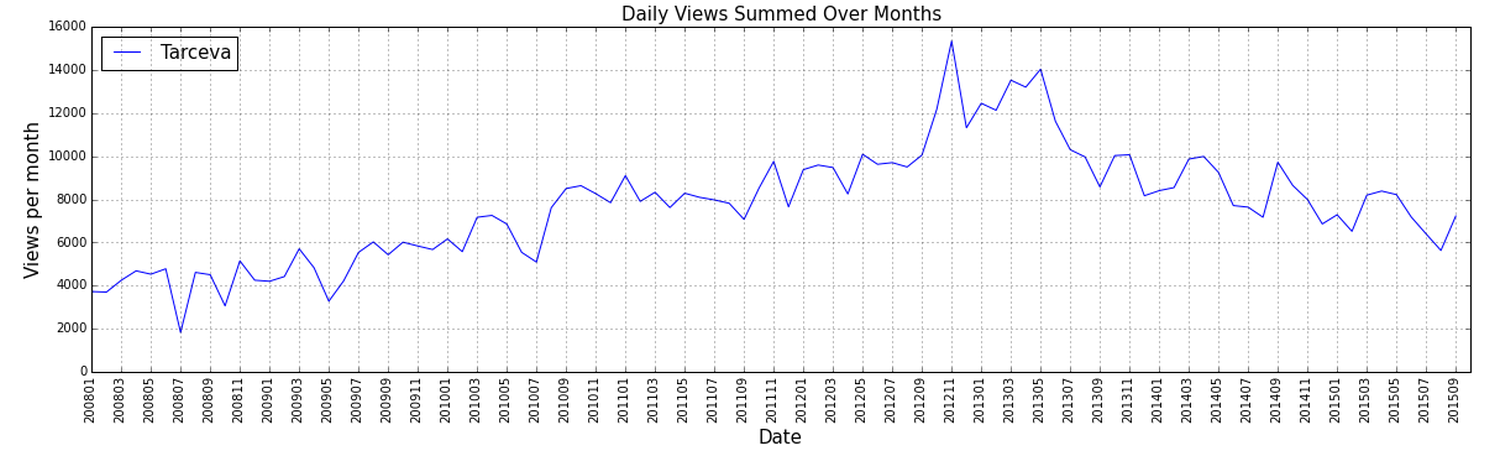
\includegraphics[scale=0.3]{tarceva_plot.png}

This notebook uses Wikipedia page views as a souce of time series data.
The reason I'm so interested in WP, is that it may be a proxy for other
other media channel interest.

For instance, what has been the national interest on the cancer
treatment drug Tarceva. It's difficult to get a long history consumer of
content from Twitter, Youtube, Facebook, etc. Wikipedia offers a full
seven years of basic usage stats.

I have three goals with this notebook:

\begin{itemize}
\itemsep1pt\parskip0pt\parsep0pt
\item
  Show how to pull view data from Wikipedia
\item
  Provide examples of signal processing of time series
\item
  Understand the behavior of Wikipedia users (content viewers)
\end{itemize}

In addition, the contributor's stats on edits is available. That also
might yield some interesting analysis. For instance the page maintainers
for a drug, might well be a key influencer in the field. Or, the time
series data which belongs to an editor, might be used as a co-variate to
be removed. Perhaps the amount of time a competitor company puts into
their WP article will provide insight for a client.

\paragraph{For now, let's restrict ourselves to page
views.}\label{for-now-lets-restrict-ourselves-to-page-views.}

    \subsection{Version Information}\label{version-information}

https://github.com/rasbt/watermark

    \begin{Verbatim}[commandchars=\\\{\}]
{\color{incolor}In [{\color{incolor}1}]:} \PY{o}{\PYZpc{}}\PY{k}{load\PYZus{}ext} watermark
        \PY{o}{\PYZpc{}}\PY{k}{watermark} \PYZhy{}g \PYZhy{}p numpy,scipy,pandas,matplotlib,statsmodels
\end{Verbatim}

    \begin{Verbatim}[commandchars=\\\{\}]
numpy 1.10.1
scipy 0.16.0
pandas 0.16.2
matplotlib 1.4.0
statsmodels 0.6.1
Git hash: 6d0545dbff99640dde1cee14c3d90b107d98c24c
    \end{Verbatim}

    \subsection{Core Logic For Downloading the
Data}\label{core-logic-for-downloading-the-data}

    \begin{Verbatim}[commandchars=\\\{\}]
{\color{incolor}In [{\color{incolor}1}]:} \PY{o}{\PYZpc{}}\PY{k}{matplotlib} inline
        \PY{c}{\PYZsh{} this sets up the default fig size}
        \PY{k+kn}{from} \PY{n+nn}{matplotlib} \PY{k+kn}{import} \PY{n}{rcParams}
        \PY{n}{rcParams}\PY{p}{[}\PY{l+s}{\PYZsq{}}\PY{l+s}{figure.figsize}\PY{l+s}{\PYZsq{}}\PY{p}{]} \PY{o}{=} \PY{p}{(}\PY{l+m+mi}{20}\PY{p}{,} \PY{l+m+mi}{5}\PY{p}{)}
        \PY{k+kn}{import} \PY{n+nn}{urllib2}
        \PY{k+kn}{import} \PY{n+nn}{pandas} \PY{k+kn}{as} \PY{n+nn}{pd}
        \PY{k+kn}{import} \PY{n+nn}{numpy} \PY{k+kn}{as} \PY{n+nn}{np}
        \PY{k+kn}{import} \PY{n+nn}{scipy.signal}
        \PY{k+kn}{import} \PY{n+nn}{matplotlib.pyplot} \PY{k+kn}{as} \PY{n+nn}{plt}
        \PY{k+kn}{import} \PY{n+nn}{json}
        \PY{k+kn}{from} \PY{n+nn}{time} \PY{k+kn}{import} \PY{n}{sleep}

        \PY{k}{class} \PY{n+nc}{WikiViews}\PY{p}{(}\PY{n+nb}{object}\PY{p}{)}\PY{p}{:}
            \PY{k}{def} \PY{n+nf}{\PYZus{}\PYZus{}init\PYZus{}\PYZus{}}\PY{p}{(}\PY{n+nb+bp}{self}\PY{p}{,} \PY{n}{url}\PY{p}{,} \PY{n}{start\PYZus{}date}\PY{p}{,} \PY{n}{end\PYZus{}date}\PY{p}{)}\PY{p}{:}
                \PY{n+nb+bp}{self}\PY{o}{.}\PY{n}{url} \PY{o}{=} \PY{n}{url}
                \PY{n+nb+bp}{self}\PY{o}{.}\PY{n}{url\PYZus{}base} \PY{o}{=} \PY{l+s}{\PYZdq{}}\PY{l+s}{http://stats.grok.se/json/en/}\PY{l+s+si}{\PYZpc{}(date)s}\PY{l+s}{/}\PY{l+s+si}{\PYZpc{}(url)s}\PY{l+s}{\PYZdq{}}
                \PY{n+nb+bp}{self}\PY{o}{.}\PY{n}{date\PYZus{}range} \PY{o}{=} \PY{n}{pd}\PY{o}{.}\PY{n}{date\PYZus{}range}\PY{p}{(}\PY{n}{start}\PY{o}{=}\PY{n}{start\PYZus{}date}\PY{p}{,} \PY{n}{end}\PY{o}{=}\PY{n}{end\PYZus{}date}\PY{p}{,} \PY{n}{freq}\PY{o}{=}\PY{l+s}{\PYZsq{}}\PY{l+s}{m}\PY{l+s}{\PYZsq{}}\PY{p}{)}
                \PY{n+nb+bp}{self}\PY{o}{.}\PY{n}{try\PYZus{}max} \PY{o}{=} \PY{l+m+mi}{3}
                \PY{n+nb+bp}{self}\PY{o}{.}\PY{n}{show\PYZus{}url\PYZus{}fails} \PY{o}{=} \PY{n+nb+bp}{False}

            \PY{k}{def} \PY{n+nf}{\PYZus{}get\PYZus{}data}\PY{p}{(}\PY{n+nb+bp}{self}\PY{p}{,} \PY{n}{url}\PY{p}{,} \PY{n}{try\PYZus{}num}\PY{p}{)}\PY{p}{:}
                \PY{k}{if} \PY{n}{try\PYZus{}num} \PY{o}{\PYZgt{}} \PY{n+nb+bp}{self}\PY{o}{.}\PY{n}{try\PYZus{}max}\PY{p}{:}
                    \PY{k}{print} \PY{l+s}{\PYZdq{}}\PY{l+s}{reached max try}\PY{l+s}{\PYZsq{}}\PY{l+s}{s}\PY{l+s}{\PYZdq{}}
                    \PY{k}{return} \PY{n+nb+bp}{None}
                \PY{k}{try}\PY{p}{:}
                    \PY{n}{response} \PY{o}{=} \PY{n}{urllib2}\PY{o}{.}\PY{n}{urlopen}\PY{p}{(}\PY{n}{url}\PY{p}{)}
                    \PY{n}{out} \PY{o}{=} \PY{n}{response}\PY{o}{.}\PY{n}{read}\PY{p}{(}\PY{p}{)}
                    \PY{k}{return} \PY{n}{out}
                \PY{k}{except} \PY{n}{urllib2}\PY{o}{.}\PY{n}{HTTPError}\PY{p}{:}
                    \PY{n}{sleep}\PY{p}{(}\PY{l+m+mi}{5}\PY{p}{)}
                    \PY{n}{try\PYZus{}num} \PY{o}{+}\PY{o}{=} \PY{l+m+mi}{1}
                    \PY{k}{if} \PY{n+nb+bp}{self}\PY{o}{.}\PY{n}{show\PYZus{}url\PYZus{}fails}\PY{p}{:}
                        \PY{k}{print} \PY{l+s}{\PYZdq{}}\PY{l+s}{try again:}\PY{l+s+si}{\PYZpc{}i}\PY{l+s}{:}\PY{l+s+si}{\PYZpc{}s}\PY{l+s}{\PYZdq{}} \PY{o}{\PYZpc{}}\PY{p}{(}\PY{n}{try\PYZus{}num}\PY{p}{,} \PY{n}{url}\PY{p}{)}
                    \PY{n+nb+bp}{self}\PY{o}{.}\PY{n}{\PYZus{}get\PYZus{}data}\PY{p}{(}\PY{n}{url}\PY{p}{,} \PY{n}{try\PYZus{}num}\PY{p}{)}

            \PY{k}{def} \PY{n+nf}{loop\PYZus{}over\PYZus{}dates}\PY{p}{(}\PY{n+nb+bp}{self}\PY{p}{)}\PY{p}{:}
                \PY{n}{DF} \PY{o}{=} \PY{n}{pd}\PY{o}{.}\PY{n}{DataFrame}\PY{p}{(}\PY{p}{)}

                \PY{k}{for} \PY{n}{date} \PY{o+ow}{in} \PY{n+nb+bp}{self}\PY{o}{.}\PY{n}{date\PYZus{}range}\PY{p}{:}
                    \PY{n}{date\PYZus{}string} \PY{o}{=} \PY{n}{date}\PY{o}{.}\PY{n}{strftime}\PY{p}{(}\PY{l+s}{\PYZdq{}}\PY{l+s}{\PYZpc{}}\PY{l+s}{Y}\PY{l+s}{\PYZpc{}}\PY{l+s}{m}\PY{l+s}{\PYZdq{}}\PY{p}{)}
                    \PY{n}{url} \PY{o}{=} \PY{n+nb+bp}{self}\PY{o}{.}\PY{n}{url\PYZus{}base} \PY{o}{\PYZpc{}}\PY{p}{\PYZob{}}\PY{l+s}{\PYZsq{}}\PY{l+s}{date}\PY{l+s}{\PYZsq{}}\PY{p}{:}\PY{n}{date\PYZus{}string}\PY{p}{,}
                                          \PY{l+s}{\PYZsq{}}\PY{l+s}{url}\PY{l+s}{\PYZsq{}}\PY{p}{:}\PY{n+nb+bp}{self}\PY{o}{.}\PY{n}{url}
                                          \PY{p}{\PYZcb{}}
                    \PY{k}{try}\PY{p}{:}
                        \PY{n}{try\PYZus{}num} \PY{o}{=} \PY{l+m+mi}{0}
                        \PY{n}{out} \PY{o}{=} \PY{n+nb+bp}{self}\PY{o}{.}\PY{n}{\PYZus{}get\PYZus{}data}\PY{p}{(}\PY{n}{url}\PY{p}{,} \PY{n}{try\PYZus{}num}\PY{p}{)}
                        \PY{k}{if} \PY{n}{out} \PY{o+ow}{is} \PY{n+nb+bp}{None}\PY{p}{:}
                            \PY{k}{continue}

                    \PY{k}{except} \PY{n+ne}{Exception}\PY{p}{,} \PY{n}{err}\PY{p}{:} \PY{c}{\PYZsh{} modicum of trouble shooting}
                        \PY{k}{print} \PY{n}{err}          \PY{c}{\PYZsh{} mystery failures}
                        \PY{k}{continue}
                        \PY{c}{\PYZsh{}raise Exception}

                    \PY{n}{out} \PY{o}{=} \PY{n}{json}\PY{o}{.}\PY{n}{loads}\PY{p}{(}\PY{n}{out}\PY{p}{)} \PY{c}{\PYZsh{} first column happens to be a date string, which will become the index}
                    \PY{n}{df} \PY{o}{=} \PY{n}{pd}\PY{o}{.}\PY{n}{DataFrame}\PY{p}{(}\PY{n}{out}\PY{p}{)}

                    \PY{n}{DF} \PY{o}{=} \PY{n}{DF}\PY{o}{.}\PY{n}{append}\PY{p}{(}\PY{n}{df}\PY{p}{)}
                    \PY{n}{DF} \PY{o}{=} \PY{n}{DF}\PY{o}{.}\PY{n}{reindex}\PY{p}{(}\PY{n}{fill\PYZus{}value}\PY{o}{=}\PY{l+m+mi}{0}\PY{p}{)} \PY{c}{\PYZsh{} make sure that all days are filled for later comparison}

                \PY{n}{DF}\PY{p}{[}\PY{l+s}{\PYZsq{}}\PY{l+s}{date}\PY{l+s}{\PYZsq{}}\PY{p}{]} \PY{o}{=} \PY{n}{DF}\PY{o}{.}\PY{n}{index} \PY{c}{\PYZsh{} useful when loading the data from csv file}
                \PY{k}{return} \PY{n}{DF}

            \PY{n+nd}{@classmethod} \PY{c}{\PYZsh{} shouldn\PYZsq{}t need class instance for this but it nice to keep organized in one place}
            \PY{k}{def} \PY{n+nf}{plot\PYZus{}time\PYZus{}series}\PY{p}{(}\PY{n+nb+bp}{self}\PY{p}{,} \PY{n}{df}\PY{p}{,} \PY{n}{norm}\PY{o}{=}\PY{n+nb+bp}{False}\PY{p}{)}\PY{p}{:}
                \PY{l+s+sd}{\PYZsq{}\PYZsq{}\PYZsq{}Plot time series average per month and print labels \PYZsq{}\PYZsq{}\PYZsq{}}
                \PY{n}{grp} \PY{o}{=} \PY{n}{df}\PY{o}{.}\PY{n}{groupby}\PY{p}{(}\PY{l+s}{\PYZsq{}}\PY{l+s}{month}\PY{l+s}{\PYZsq{}}\PY{p}{)}
                \PY{n}{y} \PY{o}{=} \PY{n}{grp}\PY{o}{.}\PY{n}{sum}\PY{p}{(}\PY{p}{)}

                \PY{k}{if} \PY{l+s}{\PYZsq{}}\PY{l+s}{daily\PYZus{}views}\PY{l+s}{\PYZsq{}} \PY{o+ow}{in} \PY{n}{y}\PY{o}{.}\PY{n}{keys}\PY{p}{(}\PY{p}{)}\PY{p}{:} \PY{c}{\PYZsh{} case when df is a single output of loop\PYZus{}over\PYZus{}dates}
                    \PY{n}{y} \PY{o}{=} \PY{n}{y}\PY{p}{[}\PY{l+s}{\PYZsq{}}\PY{l+s}{daily\PYZus{}views}\PY{l+s}{\PYZsq{}}\PY{p}{]}
                \PY{k}{else}\PY{p}{:}                         \PY{c}{\PYZsh{} case for df concatenation}
                    \PY{k}{pass}

                \PY{k}{if} \PY{n}{norm}\PY{p}{:}
                    \PY{n}{y} \PY{o}{/}\PY{o}{=} \PY{n}{np}\PY{o}{.}\PY{n}{std}\PY{p}{(}\PY{n}{y}\PY{p}{)}

                \PY{n}{plt}\PY{o}{.}\PY{n}{plot}\PY{p}{(}\PY{n}{y}\PY{p}{)}
                \PY{n}{plt}\PY{o}{.}\PY{n}{grid}\PY{p}{(}\PY{n+nb+bp}{True}\PY{p}{)}
                \PY{n}{plt}\PY{o}{.}\PY{n}{title}\PY{p}{(}\PY{l+s}{\PYZdq{}}\PY{l+s}{Daily Views Summed Over Months}\PY{l+s}{\PYZdq{}}\PY{p}{,} \PY{n}{fontsize}\PY{o}{=}\PY{l+m+mi}{15}\PY{p}{)}
                \PY{n}{plt}\PY{o}{.}\PY{n}{ylabel}\PY{p}{(}\PY{l+s}{\PYZdq{}}\PY{l+s}{Views per month}\PY{l+s}{\PYZdq{}}\PY{p}{,} \PY{n}{fontsize}\PY{o}{=}\PY{l+m+mi}{15}\PY{p}{)}
                \PY{n}{plt}\PY{o}{.}\PY{n}{xlabel}\PY{p}{(}\PY{l+s}{\PYZdq{}}\PY{l+s}{Date}\PY{l+s}{\PYZdq{}}\PY{p}{,} \PY{n}{fontsize}\PY{o}{=}\PY{l+m+mi}{15}\PY{p}{)}
                \PY{n}{plt}\PY{o}{.}\PY{n}{xlim}\PY{p}{(}\PY{l+m+mi}{0}\PY{p}{,} \PY{n}{y}\PY{o}{.}\PY{n}{shape}\PY{p}{[}\PY{l+m+mi}{0}\PY{p}{]}\PY{p}{)}

                \PY{n}{interval} \PY{o}{=} \PY{l+m+mi}{2}
                \PY{n}{labels} \PY{o}{=} \PY{n}{df}\PY{o}{.}\PY{n}{month}\PY{o}{.}\PY{n}{unique}\PY{p}{(}\PY{p}{)}
                \PY{n}{labels} \PY{o}{=} \PY{n}{labels}\PY{p}{[}\PY{l+m+mi}{0}\PY{p}{:}\PY{p}{:}\PY{n}{interval}\PY{p}{]}

                \PY{n}{n} \PY{o}{=} \PY{n}{np}\PY{o}{.}\PY{n}{arange}\PY{p}{(}\PY{n+nb}{len}\PY{p}{(}\PY{n}{y}\PY{p}{)}\PY{p}{)}\PY{p}{[}\PY{l+m+mi}{0}\PY{p}{:}\PY{p}{:}\PY{n}{interval}\PY{p}{]}
                \PY{n}{plt}\PY{o}{.}\PY{n}{xticks}\PY{p}{(}\PY{n}{n}\PY{p}{,} \PY{n}{labels}\PY{p}{,} \PY{n}{rotation}\PY{o}{=}\PY{l+s}{\PYZsq{}}\PY{l+s}{vertical}\PY{l+s}{\PYZsq{}}\PY{p}{)}

            \PY{n+nd}{@classmethod}
            \PY{k}{def} \PY{n+nf}{fft}\PY{p}{(}\PY{n+nb+bp}{self}\PY{p}{,} \PY{n}{data}\PY{p}{)}\PY{p}{:}
                \PY{l+s+sd}{\PYZsq{}\PYZsq{}\PYZsq{}Plot FFT using Welch\PYZsq{}s method, daily resolution \PYZsq{}\PYZsq{}\PYZsq{}}
                \PY{c}{\PYZsh{}plt.figure(figsize=(13, 7))}
                \PY{n}{f}\PY{p}{,} \PY{n}{y} \PY{o}{=} \PY{n}{scipy}\PY{o}{.}\PY{n}{signal}\PY{o}{.}\PY{n}{welch}\PY{p}{(}\PY{n}{data}\PY{p}{,} \PY{n}{fs}\PY{o}{=}\PY{l+m+mf}{1.0}\PY{p}{,} \PY{n}{nperseg}\PY{o}{=}\PY{l+m+mi}{256}\PY{p}{,} \PY{n}{noverlap}\PY{o}{=}\PY{l+m+mi}{128}\PY{p}{,} \PY{n}{nfft}\PY{o}{=}\PY{l+m+mi}{512}\PY{p}{,} \PY{n}{scaling}\PY{o}{=}\PY{l+s}{\PYZsq{}}\PY{l+s}{spectrum}\PY{l+s}{\PYZsq{}}\PY{p}{,} \PY{n}{detrend}\PY{o}{=}\PY{l+s}{\PYZdq{}}\PY{l+s}{linear}\PY{l+s}{\PYZdq{}}\PY{p}{)}

                \PY{n}{interval} \PY{o}{=} \PY{l+m+mi}{3} \PY{c}{\PYZsh{} days}
                \PY{n}{periods} \PY{o}{=} \PY{n}{np}\PY{o}{.}\PY{n}{round}\PY{p}{(}\PY{l+m+mi}{1}\PY{o}{/}\PY{n}{f}\PY{p}{[}\PY{l+m+mi}{0}\PY{p}{:}\PY{p}{:}\PY{n}{interval}\PY{p}{]}\PY{p}{,} \PY{l+m+mi}{1}\PY{p}{)}
                \PY{c}{\PYZsh{} clean up frequency of 0 Hz}
                \PY{n}{periods}\PY{p}{[}\PY{l+m+mi}{0}\PY{p}{]} \PY{o}{=} \PY{l+m+mi}{0}

                \PY{n}{frqs} \PY{o}{=} \PY{n}{f}\PY{p}{[}\PY{l+m+mi}{0}\PY{p}{:}\PY{p}{:}\PY{n}{interval}\PY{p}{]}
                \PY{n}{plt}\PY{o}{.}\PY{n}{xticks}\PY{p}{(}\PY{n}{frqs}\PY{p}{,} \PY{n}{periods}\PY{p}{,} \PY{n}{rotation}\PY{o}{=}\PY{l+s}{\PYZdq{}}\PY{l+s}{vertical}\PY{l+s}{\PYZdq{}}\PY{p}{)}

                \PY{n}{plt}\PY{o}{.}\PY{n}{plot}\PY{p}{(}\PY{n}{f}\PY{p}{,} \PY{n}{y}\PY{p}{)}

                \PY{n}{plt}\PY{o}{.}\PY{n}{grid}\PY{p}{(}\PY{n+nb+bp}{True}\PY{p}{)} \PY{c}{\PYZsh{} not working likely b/c of conflict with seaborn artist}
                \PY{n}{plt}\PY{o}{.}\PY{n}{title}\PY{p}{(}\PY{l+s}{\PYZdq{}}\PY{l+s}{Welch FFT: Wiki Views}\PY{l+s}{\PYZdq{}}\PY{p}{)}
                \PY{n}{plt}\PY{o}{.}\PY{n}{ylabel}\PY{p}{(}\PY{l+s}{\PYZdq{}}\PY{l+s}{Relative ratio of spectrum}\PY{l+s}{\PYZdq{}}\PY{p}{)}
                \PY{n}{plt}\PY{o}{.}\PY{n}{xlabel}\PY{p}{(}\PY{l+s}{\PYZdq{}}\PY{l+s}{Number of days in a period}\PY{l+s}{\PYZdq{}}\PY{p}{)}

                \PY{k}{return} \PY{n}{f}\PY{p}{,} \PY{n}{y}\PY{p}{,} \PY{n}{frqs}
\end{Verbatim}

    \subsection{Getting the Tarceva Stats}\label{getting-the-tarceva-stats}

This will take a while. You may wish to change the \emph{start} and
\emph{end} dates in the next cell to move through faster. Later in the
notebook I save all the pulls to csv which causes some annoyance in the
form of extra code. You may wish to selectively run each cell rather
than \emph{run all}.

It's important to note, that Tarceva is the trade name for
\emph{Erlotinib Hydrochloride}. The Wikipedia page view stats do not
always use the original article name. This is true in the case of the
Tarceva page, where the page view stats use the \emph{Erlotinib} name in
the URL. This occurs again with \emph{Iressa}, which is described below.

    \begin{Verbatim}[commandchars=\\\{\}]
{\color{incolor}In [{\color{incolor} }]:} \PY{c}{\PYZsh{} setup constants for dates of the query }
        \PY{n}{start} \PY{o}{=} \PY{l+s}{\PYZsq{}}\PY{l+s}{1/1/2008}\PY{l+s}{\PYZsq{}}
        \PY{n}{end} \PY{o}{=} \PY{l+s}{\PYZsq{}}\PY{l+s}{10/1/2015}\PY{l+s}{\PYZsq{}}
\end{Verbatim}

    \begin{Verbatim}[commandchars=\\\{\}]
{\color{incolor}In [{\color{incolor}280}]:} \PY{n}{wv} \PY{o}{=} \PY{n}{WikiViews}\PY{p}{(}\PY{l+s}{\PYZdq{}}\PY{l+s}{Erlotinib}\PY{l+s}{\PYZdq{}}\PY{p}{,} \PY{n}{start}\PY{p}{,} \PY{n}{end} \PY{p}{)}
          \PY{n}{tar} \PY{o}{=} \PY{n}{wv}\PY{o}{.}\PY{n}{loop\PYZus{}over\PYZus{}dates}\PY{p}{(}\PY{p}{)}
\end{Verbatim}

    \begin{Verbatim}[commandchars=\\\{\}]
{\color{incolor}In [{\color{incolor}281}]:} \PY{n}{tar}\PY{o}{.}\PY{n}{head}\PY{p}{(}\PY{p}{)}
\end{Verbatim}

            \begin{Verbatim}[commandchars=\\\{\}]
{\color{outcolor}Out[{\color{outcolor}281}]:}             daily\_views   month project  rank      title        date
          2008-04-01          167  200804      en    -1  Erlotinib  2008-04-01
          2008-04-02          192  200804      en    -1  Erlotinib  2008-04-02
          2008-04-03          188  200804      en    -1  Erlotinib  2008-04-03
          2008-04-04          163  200804      en    -1  Erlotinib  2008-04-04
          2008-04-05           95  200804      en    -1  Erlotinib  2008-04-05
\end{Verbatim}

    \subsection{Time Series}\label{time-series}

The data is returned on a daily basis. I don't think that is very useful
for a first look. Most people want to see the trend. We should keep in
mind, that WP's user's have grown over the years and that may account
for some trending. We'll use signal processing techniques later that
will account for that.

    \begin{Verbatim}[commandchars=\\\{\}]
{\color{incolor}In [{\color{incolor}6}]:} \PY{n}{WikiViews}\PY{o}{.}\PY{n}{plot\PYZus{}time\PYZus{}series}\PY{p}{(}\PY{n}{tar}\PY{p}{)}
        \PY{n}{plt}\PY{o}{.}\PY{n}{legend}\PY{p}{(}\PY{p}{(}\PY{p}{[}\PY{l+s}{\PYZdq{}}\PY{l+s}{Tarceva}\PY{l+s}{\PYZdq{}}\PY{p}{]}\PY{p}{)}\PY{p}{,} \PY{n}{loc}\PY{o}{=}\PY{l+s}{\PYZdq{}}\PY{l+s}{upper left}\PY{l+s}{\PYZdq{}}\PY{p}{,} \PY{n}{fontsize}\PY{o}{=}\PY{l+m+mi}{15}\PY{p}{)}
\end{Verbatim}

            \begin{Verbatim}[commandchars=\\\{\}]
{\color{outcolor}Out[{\color{outcolor}6}]:} <matplotlib.legend.Legend at 0x7f81f85efe50>
\end{Verbatim}

    \begin{center}
    \adjustimage{max size={0.9\linewidth}{0.9\paperheight}}{wikipedia_views_files/wikipedia_views_9_1.png}
    \end{center}
    { \hspace*{\fill} \\}

    \subsection{Covariates}\label{covariates}

We'd like to be able to know what high level topics influence the
interest in the drug Tarceva. We'll look for covariates and try to come
up with some entry point ideas that we would present to a domain export
or analyst.

    We would want to talk to a domain expert about that. Of course we an do
some Google searches of our own and try to find covariates.

Google search about Tarceva turns up:

\begin{itemize}
\itemsep1pt\parskip0pt\parsep0pt
\item
  Tarvcea acts on, ``Epidermal growth factor receptor''
\item
  Tarceva is also used to treat
\item
  Non small cell lung cancer
\item
  Pancreatic cancer
\item
  Older drug named Iressa is the predecessor
\end{itemize}

Might as well do some more Wikipedia pulls, because it will be hard to
find source to cross reference in the news that covers a span of time.
Let's try more topics.

    \begin{Verbatim}[commandchars=\\\{\}]
{\color{incolor}In [{\color{incolor}34}]:} \PY{n}{wv} \PY{o}{=} \PY{n}{WikiViews}\PY{p}{(}\PY{l+s}{\PYZdq{}}\PY{l+s}{Epidermal\PYZus{}growth\PYZus{}factor\PYZus{}receptor}\PY{l+s}{\PYZdq{}}\PY{p}{,} \PY{n}{start}\PY{p}{,} \PY{n}{end} \PY{p}{)}
         \PY{n}{egfr} \PY{o}{=} \PY{n}{wv}\PY{o}{.}\PY{n}{loop\PYZus{}over\PYZus{}dates}\PY{p}{(}\PY{p}{)}
\end{Verbatim}

    \begin{Verbatim}[commandchars=\\\{\}]
{\color{incolor}In [{\color{incolor}35}]:} \PY{n}{wv} \PY{o}{=} \PY{n}{WikiViews}\PY{p}{(}\PY{l+s}{\PYZdq{}}\PY{l+s}{Lung\PYZus{}cancer}\PY{l+s}{\PYZdq{}}\PY{p}{,} \PY{n}{start}\PY{p}{,} \PY{n}{end}\PY{p}{)}
         \PY{n}{lung} \PY{o}{=} \PY{n}{wv}\PY{o}{.}\PY{n}{loop\PYZus{}over\PYZus{}dates}\PY{p}{(}\PY{p}{)}
\end{Verbatim}

    \begin{Verbatim}[commandchars=\\\{\}]
{\color{incolor}In [{\color{incolor}36}]:} \PY{n}{wv} \PY{o}{=} \PY{n}{WikiViews}\PY{p}{(}\PY{l+s}{\PYZdq{}}\PY{l+s}{Gefitinib}\PY{l+s}{\PYZdq{}}\PY{p}{,} \PY{n}{start}\PY{p}{,} \PY{n}{end}\PY{p}{)}
         \PY{n}{iressa} \PY{o}{=} \PY{n}{wv}\PY{o}{.}\PY{n}{loop\PYZus{}over\PYZus{}dates}\PY{p}{(}\PY{p}{)}
\end{Verbatim}

    \begin{Verbatim}[commandchars=\\\{\}]
{\color{incolor}In [{\color{incolor}37}]:} \PY{n}{tar}\PY{p}{[}\PY{l+s}{\PYZsq{}}\PY{l+s}{date}\PY{l+s}{\PYZsq{}}\PY{p}{]} \PY{o}{=} \PY{n}{df}\PY{o}{.}\PY{n}{index}
         \PY{n}{df} \PY{o}{=} \PY{n}{pd}\PY{o}{.}\PY{n}{concat}\PY{p}{(}\PY{p}{\PYZob{}}\PY{l+s}{\PYZsq{}}\PY{l+s}{date}\PY{l+s}{\PYZsq{}}\PY{p}{:}\PY{n}{tar}\PY{o}{.}\PY{n}{date}\PY{p}{,}
                         \PY{l+s}{\PYZsq{}}\PY{l+s}{month}\PY{l+s}{\PYZsq{}}\PY{p}{:}\PY{n}{tar}\PY{o}{.}\PY{n}{month}\PY{p}{,}
                         \PY{l+s}{\PYZsq{}}\PY{l+s}{tar}\PY{l+s}{\PYZsq{}}\PY{p}{:}\PY{n}{tar}\PY{o}{.}\PY{n}{daily\PYZus{}views}\PY{p}{,}
                         \PY{l+s}{\PYZsq{}}\PY{l+s}{egfr}\PY{l+s}{\PYZsq{}}\PY{p}{:}\PY{n}{egfr}\PY{o}{.}\PY{n}{daily\PYZus{}views}\PY{p}{,}
                         \PY{l+s}{\PYZsq{}}\PY{l+s}{lung}\PY{l+s}{\PYZsq{}}\PY{p}{:}\PY{n}{lung}\PY{o}{.}\PY{n}{daily\PYZus{}views}\PY{p}{,}
                         \PY{l+s}{\PYZsq{}}\PY{l+s}{iressa}\PY{l+s}{\PYZsq{}}\PY{p}{:}\PY{n}{iressa}\PY{o}{.}\PY{n}{daily\PYZus{}views}
                        \PY{p}{\PYZcb{}}\PY{p}{,} \PY{n}{axis}\PY{o}{=}\PY{l+m+mi}{1}\PY{p}{)}

         \PY{n}{df}\PY{o}{.}\PY{n}{to\PYZus{}csv}\PY{p}{(}\PY{l+s}{\PYZdq{}}\PY{l+s}{/home/daniel/git/Python2.7/DataScience/notebooks/wikipedia\PYZus{}views/wiki\PYZus{}views\PYZus{}data.csv}\PY{l+s}{\PYZdq{}}\PY{p}{,} \PY{n}{index}\PY{o}{=}\PY{n+nb+bp}{False}\PY{p}{)}
\end{Verbatim}

    \begin{Verbatim}[commandchars=\\\{\}]
{\color{incolor}In [{\color{incolor}39}]:} \PY{n}{df}\PY{o}{.}\PY{n}{head}\PY{p}{(}\PY{p}{)}
         \PY{n}{dfcopy} \PY{o}{=} \PY{n}{df}\PY{o}{.}\PY{n}{copy}\PY{p}{(}\PY{p}{)}
\end{Verbatim}

    I kept coming back to this notebook for work on it and didn't want to
wait for the data to download. Below I'm loading it back from a csv
file.

    \begin{Verbatim}[commandchars=\\\{\}]
{\color{incolor}In [{\color{incolor}2}]:} \PY{n}{df} \PY{o}{=} \PY{n}{pd}\PY{o}{.}\PY{n}{read\PYZus{}csv}\PY{p}{(}\PY{l+s}{\PYZdq{}}\PY{l+s}{/home/daniel/git/Python2.7/DataScience/notebooks/wikipedia\PYZus{}views/wiki\PYZus{}views\PYZus{}data.csv}\PY{l+s}{\PYZdq{}}\PY{p}{)}
        \PY{n}{df}\PY{o}{.}\PY{n}{set\PYZus{}index}\PY{p}{(}\PY{l+s}{\PYZdq{}}\PY{l+s}{date}\PY{l+s}{\PYZdq{}}\PY{p}{,} \PY{n}{drop}\PY{o}{=}\PY{n+nb+bp}{True}\PY{p}{,} \PY{n}{inplace}\PY{o}{=}\PY{n+nb+bp}{True}\PY{p}{)}
        \PY{n}{df}\PY{o}{.}\PY{n}{head}\PY{p}{(}\PY{p}{)}
\end{Verbatim}

            \begin{Verbatim}[commandchars=\\\{\}]
{\color{outcolor}Out[{\color{outcolor}2}]:}             egfr  iressa  lung   month  tar
        date
        2008-01-01    64      40  1357  200801   47
        2008-01-02   156      81  2205  200801  133
        2008-01-03   213     100  2728  200801  118
        2008-01-04   174      89  2582  200801  108
        2008-01-05    87      53  1885  200801   72
\end{Verbatim}

    Examine for correlation by eye. We need to normalize to correct for
scale. Note, the y label units will not be applicable for this plot.

    \begin{Verbatim}[commandchars=\\\{\}]
{\color{incolor}In [{\color{incolor}291}]:} \PY{n}{WikiViews}\PY{o}{.}\PY{n}{plot\PYZus{}time\PYZus{}series}\PY{p}{(}\PY{n}{df}\PY{p}{[}\PY{p}{[}\PY{l+s}{\PYZsq{}}\PY{l+s}{tar}\PY{l+s}{\PYZsq{}}\PY{p}{,} \PY{l+s}{\PYZsq{}}\PY{l+s}{lung}\PY{l+s}{\PYZsq{}}\PY{p}{,} \PY{l+s}{\PYZsq{}}\PY{l+s}{egfr}\PY{l+s}{\PYZsq{}}\PY{p}{,} \PY{l+s}{\PYZsq{}}\PY{l+s}{iressa}\PY{l+s}{\PYZsq{}}\PY{p}{,} \PY{l+s}{\PYZsq{}}\PY{l+s}{month}\PY{l+s}{\PYZsq{}}\PY{p}{]}\PY{p}{]}\PY{p}{,} \PY{n}{norm}\PY{o}{=}\PY{n+nb+bp}{True}\PY{p}{)}
          \PY{n}{plt}\PY{o}{.}\PY{n}{legend}\PY{p}{(}\PY{p}{(}\PY{l+s}{\PYZsq{}}\PY{l+s}{Lung cancer}\PY{l+s}{\PYZsq{}}\PY{p}{,} \PY{l+s}{\PYZsq{}}\PY{l+s}{Tarceva}\PY{l+s}{\PYZsq{}}\PY{p}{,} \PY{l+s}{\PYZsq{}}\PY{l+s}{EGFR}\PY{l+s}{\PYZsq{}}\PY{p}{,} \PY{l+s}{\PYZsq{}}\PY{l+s}{Iressa}\PY{l+s}{\PYZsq{}}\PY{p}{)}\PY{p}{,} \PY{n}{loc}\PY{o}{=}\PY{l+s}{\PYZdq{}}\PY{l+s}{upper left}\PY{l+s}{\PYZdq{}}\PY{p}{,} \PY{n}{fontsize}\PY{o}{=}\PY{l+m+mi}{15}\PY{p}{)}
          \PY{n}{plt}\PY{o}{.}\PY{n}{ylabel}\PY{p}{(}\PY{l+s}{\PYZdq{}}\PY{l+s}{views per month normed to std}\PY{l+s}{\PYZdq{}}\PY{p}{)}
\end{Verbatim}

            \begin{Verbatim}[commandchars=\\\{\}]
{\color{outcolor}Out[{\color{outcolor}291}]:} <matplotlib.text.Text at 0x7f193a23c650>
\end{Verbatim}

    \begin{center}
    \adjustimage{max size={0.9\linewidth}{0.9\paperheight}}{wikipedia_views_files/wikipedia_views_20_1.png}
    \end{center}
    { \hspace*{\fill} \\}

    \subsection{Correlation}\label{correlation}

Recall, this is just a very basic exercise. We are using really
obviously connected information to form a quick and dirty report
suitable for an analysis to look at on day one of a project. We will
need to search more for data which could be used to predict.

Examination by eye of the above plots, looks like all 4 topics are
roughly correlated in time. It's good to get a quantifier though.
Tarceva and Lung Cancer have a relatively small correlation compared to
EGFR.

    \begin{Verbatim}[commandchars=\\\{\}]
{\color{incolor}In [{\color{incolor}292}]:} \PY{n}{df}\PY{p}{[}\PY{p}{[}\PY{l+s}{\PYZsq{}}\PY{l+s}{tar}\PY{l+s}{\PYZsq{}}\PY{p}{,} \PY{l+s}{\PYZsq{}}\PY{l+s}{egfr}\PY{l+s}{\PYZsq{}}\PY{p}{,} \PY{l+s}{\PYZsq{}}\PY{l+s}{lung}\PY{l+s}{\PYZsq{}}\PY{p}{,} \PY{l+s}{\PYZsq{}}\PY{l+s}{iressa}\PY{l+s}{\PYZsq{}}\PY{p}{]}\PY{p}{]}\PY{o}{.}\PY{n}{corr}\PY{p}{(}\PY{p}{)}
\end{Verbatim}

            \begin{Verbatim}[commandchars=\\\{\}]
{\color{outcolor}Out[{\color{outcolor}292}]:}              tar      egfr      lung    iressa
          tar     1.000000  0.821299  0.210851  0.774580
          egfr    0.821299  1.000000  0.227172  0.872449
          lung    0.210851  0.227172  1.000000  0.235276
          iressa  0.774580  0.872449  0.235276  1.000000
\end{Verbatim}

    \subsection{GLM with statsmodels}\label{glm-with-statsmodels}

    \begin{Verbatim}[commandchars=\\\{\}]
{\color{incolor}In [{\color{incolor}293}]:} \PY{k+kn}{import} \PY{n+nn}{statsmodels.api} \PY{k+kn}{as} \PY{n+nn}{sm}
          \PY{n}{signal} \PY{o}{=} \PY{n}{df}\PY{p}{[}\PY{l+s}{\PYZsq{}}\PY{l+s}{tar}\PY{l+s}{\PYZsq{}}\PY{p}{]}
          \PY{n}{cov} \PY{o}{=} \PY{n}{df}\PY{p}{[}\PY{p}{[}\PY{l+s}{\PYZsq{}}\PY{l+s}{egfr}\PY{l+s}{\PYZsq{}}\PY{p}{,}\PY{l+s}{\PYZsq{}}\PY{l+s}{iressa}\PY{l+s}{\PYZsq{}}\PY{p}{,}\PY{l+s}{\PYZsq{}}\PY{l+s}{lung}\PY{l+s}{\PYZsq{}}\PY{p}{]}\PY{p}{]}
          \PY{n}{cov} \PY{o}{=} \PY{n}{np}\PY{o}{.}\PY{n}{asarray}\PY{p}{(}\PY{n}{cov}\PY{o}{.}\PY{n}{astype}\PY{p}{(}\PY{n}{np}\PY{o}{.}\PY{n}{float32}\PY{p}{)}\PY{p}{)}

          \PY{n}{signal} \PY{o}{=} \PY{n}{np}\PY{o}{.}\PY{n}{asarray}\PY{p}{(}\PY{n}{df}\PY{p}{[}\PY{l+s}{\PYZsq{}}\PY{l+s}{tar}\PY{l+s}{\PYZsq{}}\PY{p}{]}\PY{o}{.}\PY{n}{astype}\PY{p}{(}\PY{n}{np}\PY{o}{.}\PY{n}{float32}\PY{p}{)}\PY{p}{)}

          \PY{c}{\PYZsh{} GLM}
          \PY{n}{model} \PY{o}{=} \PY{n}{sm}\PY{o}{.}\PY{n}{GLM}\PY{p}{(}\PY{n}{signal}\PY{p}{,} \PY{n}{cov}\PY{p}{,} \PY{n}{family}\PY{o}{=}\PY{n}{sm}\PY{o}{.}\PY{n}{families}\PY{o}{.}\PY{n}{Gaussian}\PY{p}{(}\PY{p}{)}\PY{p}{)}
          \PY{n}{res} \PY{o}{=} \PY{n}{model}\PY{o}{.}\PY{n}{fit}\PY{p}{(}\PY{p}{)}

          \PY{k}{print}\PY{p}{(}\PY{n}{res}\PY{o}{.}\PY{n}{summary}\PY{p}{(}\PY{p}{)}\PY{p}{)}
\end{Verbatim}

    \begin{Verbatim}[commandchars=\\\{\}]
Generalized Linear Model Regression Results
==============================================================================
Dep. Variable:                      y   No. Observations:                 2860
Model:                            GLM   Df Residuals:                     2857
Model Family:                Gaussian   Df Model:                            2
Link Function:               identity   Scale:                   5785.60152446
Method:                          IRLS   Log-Likelihood:                -16445.
Date:                Sat, 10 Oct 2015   Deviance:                   1.6529e+07
Time:                        22:37:47   Pearson chi2:                 1.65e+07
No. Iterations:                     4
==============================================================================
                 coef    std err          z      P>|z|      [95.0\% Conf. Int.]
------------------------------------------------------------------------------
x1             0.3221      0.011     28.216      0.000         0.300     0.344
x2             0.4569      0.032     14.358      0.000         0.394     0.519
x3             0.0014      0.001      2.490      0.013         0.000     0.002
==============================================================================
    \end{Verbatim}

    \section{Moving on with numerical analysis
technics}\label{moving-on-with-numerical-analysis-technics}

\subsection{Filtering and FFT}\label{filtering-and-fft}

    Now we'd like to see some frequency anaylsis. The FFT won't tell us what
day(s) the cycles repeat on, but it will show if any periodicity exists.

Below is the time series by day, rather than by monthly sum as it was
above.

    \begin{Verbatim}[commandchars=\\\{\}]
{\color{incolor}In [{\color{incolor}295}]:} \PY{n}{tar} \PY{o}{=} \PY{n}{df}\PY{o}{.}\PY{n}{tar}
          \PY{n}{plt}\PY{o}{.}\PY{n}{plot}\PY{p}{(}\PY{n}{tar}\PY{p}{)}
          \PY{n}{plt}\PY{o}{.}\PY{n}{grid}\PY{p}{(}\PY{n+nb+bp}{True}\PY{p}{)}
          \PY{n}{plt}\PY{o}{.}\PY{n}{title}\PY{p}{(}\PY{l+s}{\PYZdq{}}\PY{l+s}{Tarceva Daily Views}\PY{l+s}{\PYZdq{}}\PY{p}{,} \PY{n}{fontsize}\PY{o}{=}\PY{l+m+mi}{15}\PY{p}{)}
          \PY{n}{plt}\PY{o}{.}\PY{n}{ylabel}\PY{p}{(}\PY{l+s}{\PYZdq{}}\PY{l+s}{number of views per day}\PY{l+s}{\PYZdq{}}\PY{p}{,} \PY{n}{fontsize}\PY{o}{=}\PY{l+m+mi}{15}\PY{p}{)}
          \PY{n}{plt}\PY{o}{.}\PY{n}{xlabel}\PY{p}{(}\PY{l+s}{\PYZdq{}}\PY{l+s}{time point (day)}\PY{l+s}{\PYZdq{}}\PY{p}{,} \PY{n}{fontsize}\PY{o}{=}\PY{l+m+mi}{15}\PY{p}{)}
\end{Verbatim}

            \begin{Verbatim}[commandchars=\\\{\}]
{\color{outcolor}Out[{\color{outcolor}295}]:} <matplotlib.text.Text at 0x7f1938bd9a10>
\end{Verbatim}

    \begin{center}
    \adjustimage{max size={0.9\linewidth}{0.9\paperheight}}{wikipedia_views_files/wikipedia_views_27_1.png}
    \end{center}
    { \hspace*{\fill} \\}

    Now the frequency analysis. Note that in the Welch's function which
produces this plot, the detending feature is set to \emph{linear}.

    \begin{Verbatim}[commandchars=\\\{\}]
{\color{incolor}In [{\color{incolor}296}]:} \PY{n}{f}\PY{p}{,} \PY{n}{y}\PY{p}{,} \PY{n}{frq} \PY{o}{=} \PY{n}{WikiViews}\PY{o}{.}\PY{n}{fft}\PY{p}{(}\PY{n}{tar}\PY{p}{)}
\end{Verbatim}

    \begin{center}
    \adjustimage{max size={0.9\linewidth}{0.9\paperheight}}{wikipedia_views_files/wikipedia_views_29_0.png}
    \end{center}
    { \hspace*{\fill} \\}

    There's a clear weekly frequency that I've seen in other social media
channels. People may look use Wikipedia on the weekends more so than
weekdays. The longer periods are interesting at about a month and three
months.

The next step would be to look for covarites to explain the time series
and the periodicity.

    \subsubsection{Filtering via
Convolution}\label{filtering-via-convolution}

 With straight numeric data from sensors ( typically voltages ), it's a
lot more straight forward to process the signals. There's sample rates,
signal to noise ratios, published bandwidths. We have none of those
helpful physical insights in this case.

    \begin{Verbatim}[commandchars=\\\{\}]
{\color{incolor}In [{\color{incolor}297}]:} \PY{k+kn}{import} \PY{n+nn}{scipy.signal} \PY{k+kn}{as} \PY{n+nn}{sig}
          \PY{n}{data} \PY{o}{=} \PY{n}{df}\PY{o}{.}\PY{n}{tar}
\end{Verbatim}

    \begin{Verbatim}[commandchars=\\\{\}]
{\color{incolor}In [{\color{incolor}298}]:} \PY{n}{window} \PY{o}{=} \PY{n}{np}\PY{o}{.}\PY{n}{hanning}\PY{p}{(}\PY{l+m+mi}{30}\PY{p}{)}
          \PY{n}{plt}\PY{o}{.}\PY{n}{figure}\PY{p}{(}\PY{n}{figsize}\PY{o}{=}\PY{p}{(}\PY{l+m+mi}{4}\PY{p}{,}\PY{l+m+mi}{4}\PY{p}{)}\PY{p}{)}
          \PY{n}{plt}\PY{o}{.}\PY{n}{plot}\PY{p}{(}\PY{n}{window}\PY{p}{)}
          \PY{n}{plt}\PY{o}{.}\PY{n}{grid}\PY{p}{(}\PY{n+nb+bp}{True}\PY{p}{)}
\end{Verbatim}

    \begin{center}
    \adjustimage{max size={0.9\linewidth}{0.9\paperheight}}{wikipedia_views_files/wikipedia_views_33_0.png}
    \end{center}
    { \hspace*{\fill} \\}

    \subsubsection{Before the Filter}\label{before-the-filter}

    \begin{Verbatim}[commandchars=\\\{\}]
{\color{incolor}In [{\color{incolor}299}]:} \PY{n}{plt}\PY{o}{.}\PY{n}{figure}\PY{p}{(}\PY{p}{)}
          \PY{n}{plt}\PY{o}{.}\PY{n}{plot}\PY{p}{(}\PY{n}{data}\PY{p}{[}\PY{l+m+mi}{0}\PY{p}{:}\PY{l+m+mi}{1000}\PY{p}{]}\PY{p}{)}
          \PY{n}{plt}\PY{o}{.}\PY{n}{grid}\PY{p}{(}\PY{n+nb+bp}{True}\PY{p}{)}
          \PY{n}{plt}\PY{o}{.}\PY{n}{title}\PY{p}{(}\PY{l+s}{\PYZdq{}}\PY{l+s}{Raw Time Series Data, first 1000 pts}\PY{l+s}{\PYZdq{}}\PY{p}{)}
\end{Verbatim}

            \begin{Verbatim}[commandchars=\\\{\}]
{\color{outcolor}Out[{\color{outcolor}299}]:} <matplotlib.text.Text at 0x7f193874d190>
\end{Verbatim}

    \begin{center}
    \adjustimage{max size={0.9\linewidth}{0.9\paperheight}}{wikipedia_views_files/wikipedia_views_35_1.png}
    \end{center}
    { \hspace*{\fill} \\}

    \subsubsection{After the Filter}\label{after-the-filter}

    \begin{Verbatim}[commandchars=\\\{\}]
{\color{incolor}In [{\color{incolor}300}]:} \PY{n}{data\PYZus{}filt\PYZus{}30} \PY{o}{=} \PY{n}{sig}\PY{o}{.}\PY{n}{fftconvolve}\PY{p}{(}\PY{n}{window}\PY{p}{,} \PY{n}{data}\PY{p}{)}

          \PY{n}{plt}\PY{o}{.}\PY{n}{plot}\PY{p}{(}\PY{n}{data\PYZus{}filt\PYZus{}30}\PY{p}{[}\PY{l+m+mi}{0}\PY{p}{:}\PY{l+m+mi}{1000}\PY{p}{]}\PY{p}{)}
          \PY{n}{plt}\PY{o}{.}\PY{n}{grid}\PY{p}{(}\PY{n+nb+bp}{True}\PY{p}{)}
          \PY{n}{plt}\PY{o}{.}\PY{n}{title}\PY{p}{(}\PY{l+s}{\PYZdq{}}\PY{l+s}{Time Series Data (1000 points) After Filtering}\PY{l+s}{\PYZdq{}}\PY{p}{)}
\end{Verbatim}

            \begin{Verbatim}[commandchars=\\\{\}]
{\color{outcolor}Out[{\color{outcolor}300}]:} <matplotlib.text.Text at 0x7f193860f2d0>
\end{Verbatim}

    \begin{center}
    \adjustimage{max size={0.9\linewidth}{0.9\paperheight}}{wikipedia_views_files/wikipedia_views_37_1.png}
    \end{center}
    { \hspace*{\fill} \\}

    \subsubsection{FFT After Filtering}\label{fft-after-filtering}

    \begin{Verbatim}[commandchars=\\\{\}]
{\color{incolor}In [{\color{incolor}301}]:} \PY{n}{freq}\PY{p}{,} \PY{n}{y}\PY{p}{,} \PY{n}{frqs} \PY{o}{=} \PY{n}{WikiViews}\PY{o}{.}\PY{n}{fft}\PY{p}{(}\PY{n}{data\PYZus{}filt\PYZus{}30}\PY{p}{)}
          \PY{n}{plt}\PY{o}{.}\PY{n}{xlim}\PY{p}{(}\PY{n}{frqs}\PY{p}{[}\PY{l+m+mi}{0}\PY{p}{]}\PY{p}{,} \PY{n}{frqs}\PY{p}{[}\PY{l+m+mi}{30}\PY{p}{]}\PY{p}{)}
\end{Verbatim}

            \begin{Verbatim}[commandchars=\\\{\}]
{\color{outcolor}Out[{\color{outcolor}301}]:} (0.0, 0.17578125)
\end{Verbatim}

    \begin{center}
    \adjustimage{max size={0.9\linewidth}{0.9\paperheight}}{wikipedia_views_files/wikipedia_views_39_1.png}
    \end{center}
    { \hspace*{\fill} \\}

    Although the peak looks bigger, there is no straight forward way to
scale the y axis so we need to not be too impressed with that. Really,
the same two peaks are present as in the original FFT. This plot is
simply cleaner. This might seem dumb, but if we where writing a
peak-detector, then we'd want a simpler data set.

    \subsection{Find peaks}\label{find-peaks}

    \subsubsection{The Savitzky-Golay filer was taken from
here:}\label{the-savitzky-golay-filer-was-taken-from-here}

http://wiki.scipy.org/Cookbook/SavitzkyGolay

    \begin{Verbatim}[commandchars=\\\{\}]
{\color{incolor}In [{\color{incolor}6}]:} \PY{k+kn}{from} \PY{n+nn}{math} \PY{k+kn}{import} \PY{n}{factorial}

        \PY{k}{def} \PY{n+nf}{savitzky\PYZus{}golay}\PY{p}{(}\PY{n}{y}\PY{p}{,} \PY{n}{window\PYZus{}size}\PY{p}{,} \PY{n}{order}\PY{p}{,} \PY{n}{deriv}\PY{o}{=}\PY{l+m+mi}{0}\PY{p}{,} \PY{n}{rate}\PY{o}{=}\PY{l+m+mi}{1}\PY{p}{)}\PY{p}{:}
            \PY{c}{\PYZsh{} usage and comments removed for brevity see the cookbook link for details}
            \PY{k}{try}\PY{p}{:}
                \PY{n}{window\PYZus{}size} \PY{o}{=} \PY{n}{np}\PY{o}{.}\PY{n}{abs}\PY{p}{(}\PY{n}{np}\PY{o}{.}\PY{n}{int}\PY{p}{(}\PY{n}{window\PYZus{}size}\PY{p}{)}\PY{p}{)}
                \PY{n}{order} \PY{o}{=} \PY{n}{np}\PY{o}{.}\PY{n}{abs}\PY{p}{(}\PY{n}{np}\PY{o}{.}\PY{n}{int}\PY{p}{(}\PY{n}{order}\PY{p}{)}\PY{p}{)}

            \PY{k}{except} \PY{n+ne}{ValueError}\PY{p}{,} \PY{n}{msg}\PY{p}{:}
                \PY{k}{raise} \PY{n+ne}{ValueError}\PY{p}{(}\PY{l+s}{\PYZdq{}}\PY{l+s}{window\PYZus{}size and order have to be of type int}\PY{l+s}{\PYZdq{}}\PY{p}{)}

            \PY{k}{if} \PY{n}{window\PYZus{}size} \PY{o}{\PYZpc{}} \PY{l+m+mi}{2} \PY{o}{!=} \PY{l+m+mi}{1} \PY{o+ow}{or} \PY{n}{window\PYZus{}size} \PY{o}{\PYZlt{}} \PY{l+m+mi}{1}\PY{p}{:}
                \PY{k}{raise} \PY{n+ne}{TypeError}\PY{p}{(}\PY{l+s}{\PYZdq{}}\PY{l+s}{window\PYZus{}size size must be a positive odd number}\PY{l+s}{\PYZdq{}}\PY{p}{)}

            \PY{k}{if} \PY{n}{window\PYZus{}size} \PY{o}{\PYZlt{}} \PY{n}{order} \PY{o}{+} \PY{l+m+mi}{2}\PY{p}{:}
                \PY{k}{raise} \PY{n+ne}{TypeError}\PY{p}{(}\PY{l+s}{\PYZdq{}}\PY{l+s}{window\PYZus{}size is too small for the polynomials order}\PY{l+s}{\PYZdq{}}\PY{p}{)}

            \PY{n}{order\PYZus{}range} \PY{o}{=} \PY{n+nb}{range}\PY{p}{(}\PY{n}{order}\PY{o}{+}\PY{l+m+mi}{1}\PY{p}{)}
            \PY{n}{half\PYZus{}window} \PY{o}{=} \PY{p}{(}\PY{n}{window\PYZus{}size} \PY{o}{\PYZhy{}}\PY{l+m+mi}{1}\PY{p}{)} \PY{o}{/}\PY{o}{/} \PY{l+m+mi}{2}

            \PY{c}{\PYZsh{} precompute coefficients}
            \PY{n}{b} \PY{o}{=} \PY{n}{np}\PY{o}{.}\PY{n}{mat}\PY{p}{(}\PY{p}{[}\PY{p}{[}\PY{n}{k}\PY{o}{*}\PY{o}{*}\PY{n}{i} \PY{k}{for} \PY{n}{i} \PY{o+ow}{in} \PY{n}{order\PYZus{}range}\PY{p}{]} \PY{k}{for} \PY{n}{k} \PY{o+ow}{in} \PY{n+nb}{range}\PY{p}{(}\PY{o}{\PYZhy{}}\PY{n}{half\PYZus{}window}\PY{p}{,} \PY{n}{half\PYZus{}window}\PY{o}{+}\PY{l+m+mi}{1}\PY{p}{)}\PY{p}{]}\PY{p}{)}
            \PY{n}{m} \PY{o}{=} \PY{n}{np}\PY{o}{.}\PY{n}{linalg}\PY{o}{.}\PY{n}{pinv}\PY{p}{(}\PY{n}{b}\PY{p}{)}\PY{o}{.}\PY{n}{A}\PY{p}{[}\PY{n}{deriv}\PY{p}{]} \PY{o}{*} \PY{n}{rate}\PY{o}{*}\PY{o}{*}\PY{n}{deriv} \PY{o}{*} \PY{n}{factorial}\PY{p}{(}\PY{n}{deriv}\PY{p}{)}

            \PY{c}{\PYZsh{} pad the signal at the extremes with}
            \PY{c}{\PYZsh{} values taken from the signal itself}
            \PY{n}{firstvals} \PY{o}{=} \PY{n}{y}\PY{p}{[}\PY{l+m+mi}{0}\PY{p}{]} \PY{o}{\PYZhy{}} \PY{n}{np}\PY{o}{.}\PY{n}{abs}\PY{p}{(} \PY{n}{y}\PY{p}{[}\PY{l+m+mi}{1}\PY{p}{:}\PY{n}{half\PYZus{}window}\PY{o}{+}\PY{l+m+mi}{1}\PY{p}{]}\PY{p}{[}\PY{p}{:}\PY{p}{:}\PY{o}{\PYZhy{}}\PY{l+m+mi}{1}\PY{p}{]} \PY{o}{\PYZhy{}} \PY{n}{y}\PY{p}{[}\PY{l+m+mi}{0}\PY{p}{]} \PY{p}{)}
            \PY{n}{lastvals} \PY{o}{=} \PY{n}{y}\PY{p}{[}\PY{o}{\PYZhy{}}\PY{l+m+mi}{1}\PY{p}{]} \PY{o}{+} \PY{n}{np}\PY{o}{.}\PY{n}{abs}\PY{p}{(}\PY{n}{y}\PY{p}{[}\PY{o}{\PYZhy{}}\PY{n}{half\PYZus{}window}\PY{o}{\PYZhy{}}\PY{l+m+mi}{1}\PY{p}{:}\PY{o}{\PYZhy{}}\PY{l+m+mi}{1}\PY{p}{]}\PY{p}{[}\PY{p}{:}\PY{p}{:}\PY{o}{\PYZhy{}}\PY{l+m+mi}{1}\PY{p}{]} \PY{o}{\PYZhy{}} \PY{n}{y}\PY{p}{[}\PY{o}{\PYZhy{}}\PY{l+m+mi}{1}\PY{p}{]}\PY{p}{)}

            \PY{n}{y} \PY{o}{=} \PY{n}{np}\PY{o}{.}\PY{n}{concatenate}\PY{p}{(}\PY{p}{(}\PY{n}{firstvals}\PY{p}{,} \PY{n}{y}\PY{p}{,} \PY{n}{lastvals}\PY{p}{)}\PY{p}{)}

            \PY{k}{return} \PY{n}{np}\PY{o}{.}\PY{n}{convolve}\PY{p}{(} \PY{n}{m}\PY{p}{[}\PY{p}{:}\PY{p}{:}\PY{o}{\PYZhy{}}\PY{l+m+mi}{1}\PY{p}{]}\PY{p}{,} \PY{n}{y}\PY{p}{,} \PY{n}{mode}\PY{o}{=}\PY{l+s}{\PYZsq{}}\PY{l+s}{valid}\PY{l+s}{\PYZsq{}}\PY{p}{)}
\end{Verbatim}

    This function is just an implementation of the first and second
derivative tests.

    \begin{Verbatim}[commandchars=\\\{\}]
{\color{incolor}In [{\color{incolor}7}]:} \PY{k}{def} \PY{n+nf}{peak\PYZus{}detection}\PY{p}{(}\PY{n}{data}\PY{p}{)}\PY{p}{:}
            \PY{n}{der1} \PY{o}{=} \PY{n}{savitzky\PYZus{}golay}\PY{p}{(}\PY{n}{data}\PY{p}{,} \PY{n}{window\PYZus{}size}\PY{o}{=}\PY{l+m+mi}{3}\PY{p}{,} \PY{n}{order}\PY{o}{=}\PY{l+m+mi}{1}\PY{p}{,} \PY{n}{deriv}\PY{o}{=}\PY{l+m+mi}{1}\PY{p}{)}
            \PY{n}{der2} \PY{o}{=} \PY{n}{savitzky\PYZus{}golay}\PY{p}{(}\PY{n}{data}\PY{p}{,} \PY{n}{window\PYZus{}size}\PY{o}{=}\PY{l+m+mi}{5}\PY{p}{,} \PY{n}{order}\PY{o}{=}\PY{l+m+mi}{2}\PY{p}{,} \PY{n}{deriv}\PY{o}{=}\PY{l+m+mi}{2}\PY{p}{)}
            \PY{n}{zero\PYZus{}crossings\PYZus{}test} \PY{o}{=} \PY{n}{der1}\PY{p}{[}\PY{l+m+mi}{0}\PY{p}{:}\PY{o}{\PYZhy{}}\PY{l+m+mi}{1}\PY{p}{]} \PY{o}{*} \PY{n}{der1}\PY{p}{[}\PY{l+m+mi}{1}\PY{p}{:}\PY{p}{]}
            \PY{n}{peaks} \PY{o}{=} \PY{n}{np}\PY{o}{.}\PY{n}{where}\PY{p}{(}\PY{p}{(}\PY{n}{der2}\PY{p}{[}\PY{l+m+mi}{0}\PY{p}{:}\PY{o}{\PYZhy{}}\PY{l+m+mi}{1}\PY{p}{]} \PY{o}{\PYZlt{}} \PY{l+m+mi}{0}\PY{p}{)} \PY{o}{\PYZam{}} \PY{p}{(}\PY{n}{zero\PYZus{}crossings\PYZus{}test} \PY{o}{\PYZlt{}} \PY{l+m+mi}{0}\PY{p}{)}\PY{p}{)}\PY{p}{[}\PY{l+m+mi}{0}\PY{p}{]}

            \PY{k}{return} \PY{n}{peaks}
\end{Verbatim}

    \begin{Verbatim}[commandchars=\\\{\}]
{\color{incolor}In [{\color{incolor}304}]:} \PY{n}{peaks} \PY{o}{=} \PY{n}{peak\PYZus{}detection}\PY{p}{(}\PY{n}{data\PYZus{}filt\PYZus{}30}\PY{p}{)}
\end{Verbatim}

    I find the peaks in the time series just to make sure it works.

    \begin{Verbatim}[commandchars=\\\{\}]
{\color{incolor}In [{\color{incolor}305}]:} \PY{n}{plt}\PY{o}{.}\PY{n}{plot}\PY{p}{(}\PY{n}{data\PYZus{}filt\PYZus{}30}\PY{p}{)}
          \PY{n}{plt}\PY{o}{.}\PY{n}{grid}\PY{p}{(}\PY{n+nb+bp}{True}\PY{p}{)}
          \PY{n}{plt}\PY{o}{.}\PY{n}{xlim}\PY{p}{(}\PY{l+m+mi}{0}\PY{p}{,} \PY{l+m+mi}{1000}\PY{p}{)}
          \PY{n}{plt}\PY{o}{.}\PY{n}{vlines}\PY{p}{(}\PY{n}{peaks}\PY{p}{,} \PY{l+m+mi}{0}\PY{p}{,} \PY{n}{data\PYZus{}filt\PYZus{}30}\PY{o}{.}\PY{n}{max}\PY{p}{(}\PY{p}{)}\PY{p}{,} \PY{l+s}{\PYZsq{}}\PY{l+s}{r}\PY{l+s}{\PYZsq{}}\PY{p}{,} \PY{n}{alpha}\PY{o}{=}\PY{l+m+mf}{0.3}\PY{p}{)}
          \PY{n}{plt}\PY{o}{.}\PY{n}{title}\PY{p}{(}\PY{l+s}{\PYZdq{}}\PY{l+s}{Wiki Views Tarceva: 30 Day Filter and Peaks in Red}\PY{l+s}{\PYZdq{}}\PY{p}{)}
          \PY{n}{plt}\PY{o}{.}\PY{n}{legend}\PY{p}{(}\PY{p}{(}\PY{l+s}{\PYZsq{}}\PY{l+s}{Tarceva Views}\PY{l+s}{\PYZsq{}}\PY{p}{,} \PY{l+s}{\PYZsq{}}\PY{l+s}{Peak}\PY{l+s}{\PYZsq{}}\PY{p}{)}\PY{p}{,} \PY{n}{loc}\PY{o}{=}\PY{l+s}{\PYZdq{}}\PY{l+s}{upper left}\PY{l+s}{\PYZdq{}}\PY{p}{,} \PY{n}{fontsize}\PY{o}{=}\PY{l+m+mi}{15}\PY{p}{)}
\end{Verbatim}

            \begin{Verbatim}[commandchars=\\\{\}]
{\color{outcolor}Out[{\color{outcolor}305}]:} <matplotlib.legend.Legend at 0x7f19382d46d0>
\end{Verbatim}

    \begin{center}
    \adjustimage{max size={0.9\linewidth}{0.9\paperheight}}{wikipedia_views_files/wikipedia_views_48_1.png}
    \end{center}
    { \hspace*{\fill} \\}

    Finding peaks is more useful when analyzing an FFT output.

    \begin{Verbatim}[commandchars=\\\{\}]
{\color{incolor}In [{\color{incolor}306}]:} \PY{n}{peaks} \PY{o}{=} \PY{n}{peak\PYZus{}detection}\PY{p}{(}\PY{n}{y}\PY{p}{)}
          \PY{n}{plt}\PY{o}{.}\PY{n}{figure}\PY{p}{(}\PY{p}{)}
          \PY{n}{freq}\PY{p}{,} \PY{n}{y}\PY{p}{,} \PY{n}{frqs} \PY{o}{=} \PY{n}{WikiViews}\PY{o}{.}\PY{n}{fft}\PY{p}{(}\PY{n}{data\PYZus{}filt\PYZus{}30}\PY{p}{)}
          \PY{n}{plt}\PY{o}{.}\PY{n}{vlines}\PY{p}{(}\PY{n}{freq}\PY{p}{[}\PY{n}{peaks}\PY{p}{]}\PY{p}{,} \PY{l+m+mi}{0}\PY{p}{,} \PY{n}{y}\PY{o}{.}\PY{n}{max}\PY{p}{(}\PY{p}{)}\PY{p}{,} \PY{l+s}{\PYZsq{}}\PY{l+s}{r}\PY{l+s}{\PYZsq{}}\PY{p}{)}
          \PY{n}{plt}\PY{o}{.}\PY{n}{legend}\PY{p}{(}\PY{p}{(}\PY{l+s}{\PYZsq{}}\PY{l+s}{Tarceva Views}\PY{l+s}{\PYZsq{}}\PY{p}{,} \PY{l+s}{\PYZsq{}}\PY{l+s}{Peak}\PY{l+s}{\PYZsq{}}\PY{p}{)}\PY{p}{,} \PY{n}{fontsize}\PY{o}{=}\PY{l+m+mi}{15}\PY{p}{)}
\end{Verbatim}

            \begin{Verbatim}[commandchars=\\\{\}]
{\color{outcolor}Out[{\color{outcolor}306}]:} <matplotlib.legend.Legend at 0x7f193846e350>
\end{Verbatim}

    \begin{center}
    \adjustimage{max size={0.9\linewidth}{0.9\paperheight}}{wikipedia_views_files/wikipedia_views_50_1.png}
    \end{center}
    { \hspace*{\fill} \\}

    \subsubsection{Threshold the Peaks}\label{threshold-the-peaks}

That ripple is most likely just noise from the convolution of delta
function during sampling with the actual signal.

The odd harmonics are carried over by the Convolution-Theorm. Using
Welch's method helps but does not elleviate the issue.

    \begin{Verbatim}[commandchars=\\\{\}]
{\color{incolor}In [{\color{incolor}8}]:} \PY{k}{def} \PY{n+nf}{thres\PYZus{}peaks}\PY{p}{(}\PY{n}{f}\PY{p}{,}\PY{n}{y}\PY{p}{)}\PY{p}{:}
            \PY{n}{peaks} \PY{o}{=} \PY{n}{peak\PYZus{}detection}\PY{p}{(}\PY{n}{y}\PY{p}{)}
            \PY{n}{max\PYZus{}pk} \PY{o}{=} \PY{n}{np}\PY{o}{.}\PY{n}{mean}\PY{p}{(}\PY{n}{y}\PY{p}{[}\PY{n}{peaks}\PY{p}{]}\PY{p}{)}
            \PY{n}{thres} \PY{o}{=} \PY{n}{np}\PY{o}{.}\PY{n}{where}\PY{p}{(}\PY{p}{(}\PY{n}{y}\PY{p}{[}\PY{n}{peaks}\PY{p}{]} \PY{o}{\PYZgt{}}\PY{o}{=} \PY{n}{max\PYZus{}pk}\PY{p}{)}\PY{p}{)}\PY{p}{[}\PY{l+m+mi}{0}\PY{p}{]}
            \PY{k}{return} \PY{n}{f}\PY{p}{[}\PY{n}{peaks}\PY{p}{[}\PY{n}{thres}\PY{p}{]}\PY{p}{]}
\end{Verbatim}

    \begin{Verbatim}[commandchars=\\\{\}]
{\color{incolor}In [{\color{incolor}308}]:} \PY{n}{f}\PY{p}{,} \PY{n}{y}\PY{p}{,} \PY{n}{frqs} \PY{o}{=} \PY{n}{WikiViews}\PY{o}{.}\PY{n}{fft}\PY{p}{(}\PY{n}{data\PYZus{}filt\PYZus{}30}\PY{p}{)}
          \PY{n}{fp} \PY{o}{=} \PY{n}{thres\PYZus{}peaks}\PY{p}{(}\PY{n}{f}\PY{p}{,} \PY{n}{y}\PY{p}{)}
          \PY{n}{plt}\PY{o}{.}\PY{n}{vlines}\PY{p}{(}\PY{n}{fp}\PY{p}{,} \PY{l+m+mi}{0}\PY{p}{,} \PY{n}{y}\PY{o}{.}\PY{n}{max}\PY{p}{(}\PY{p}{)}\PY{p}{,} \PY{l+s}{\PYZsq{}}\PY{l+s}{r}\PY{l+s}{\PYZsq{}}\PY{p}{)}
          \PY{n}{plt}\PY{o}{.}\PY{n}{xlim}\PY{p}{(}\PY{n}{frqs}\PY{p}{[}\PY{l+m+mi}{0}\PY{p}{]}\PY{p}{,} \PY{n}{frqs}\PY{p}{[}\PY{l+m+mi}{30}\PY{p}{]}\PY{p}{)}
          \PY{n}{plt}\PY{o}{.}\PY{n}{legend}\PY{p}{(}\PY{p}{(}\PY{l+s}{\PYZsq{}}\PY{l+s}{Tarceva Views}\PY{l+s}{\PYZsq{}}\PY{p}{,} \PY{l+s}{\PYZsq{}}\PY{l+s}{Peak}\PY{l+s}{\PYZsq{}}\PY{p}{)}\PY{p}{)}
\end{Verbatim}

            \begin{Verbatim}[commandchars=\\\{\}]
{\color{outcolor}Out[{\color{outcolor}308}]:} <matplotlib.legend.Legend at 0x7f193818b610>
\end{Verbatim}

    \begin{center}
    \adjustimage{max size={0.9\linewidth}{0.9\paperheight}}{wikipedia_views_files/wikipedia_views_53_1.png}
    \end{center}
    { \hspace*{\fill} \\}

    \subsection{Print the periods of
interest}\label{print-the-periods-of-interest}

    \begin{Verbatim}[commandchars=\\\{\}]
{\color{incolor}In [{\color{incolor}20}]:} \PY{k}{def} \PY{n+nf}{print\PYZus{}fft\PYZus{}periods}\PY{p}{(}\PY{n}{fp}\PY{p}{)}\PY{p}{:}
             \PY{n}{p} \PY{o}{=} \PY{n}{np}\PY{o}{.}\PY{n}{round}\PY{p}{(}\PY{l+m+mi}{1}\PY{o}{/}\PY{n}{fp}\PY{p}{,} \PY{n}{decimals}\PY{o}{=}\PY{l+m+mi}{1}\PY{p}{)}
             \PY{n}{pp} \PY{o}{=} \PY{l+s}{\PYZdq{}}\PY{l+s}{ days}\PY{l+s+se}{\PYZbs{}n}\PY{l+s}{ }\PY{l+s}{\PYZdq{}}\PY{o}{.}\PY{n}{join}\PY{p}{(}\PY{n+nb}{map}\PY{p}{(}\PY{n+nb}{str}\PY{p}{,} \PY{n}{p}\PY{p}{)}\PY{p}{)}
             \PY{k}{print} \PY{l+s}{\PYZdq{}}\PY{l+s}{The periods of interest are:}\PY{l+s+se}{\PYZbs{}n}\PY{l+s+si}{\PYZpc{}s}\PY{l+s}{ days}\PY{l+s}{\PYZdq{}} \PY{o}{\PYZpc{}}\PY{k}{pp}
\end{Verbatim}

    \begin{Verbatim}[commandchars=\\\{\}]
{\color{incolor}In [{\color{incolor}310}]:} \PY{n}{print\PYZus{}fft\PYZus{}periods}\PY{p}{(}\PY{n}{fp}\PY{p}{)}
\end{Verbatim}

    \begin{Verbatim}[commandchars=\\\{\}]
The periods of interest are:
170.7 days
 32.0 days
    \end{Verbatim}

    \subsection{Get Random Pages}\label{get-random-pages}

I'd like to see if there's a general viewing trend with Wikipedia. To do
that, I'll need to select pages at random. Mediawiki has an api for that
and there's a button on the Wikipedia homepage.

\emph{I didn't realize there is a rest api for Wikipedia before I wrote
this. I'm leaving it in place since it's a decent regex hack.}

    \begin{Verbatim}[commandchars=\\\{\}]
{\color{incolor}In [{\color{incolor}238}]:} \PY{k+kn}{import} \PY{n+nn}{re}
          \PY{n}{obj} \PY{o}{=} \PY{n}{re}\PY{o}{.}\PY{n}{compile}\PY{p}{(}\PY{l+s}{r\PYZsq{}}\PY{l+s}{\PYZdq{}}\PY{l+s}{wgPageName}\PY{l+s}{\PYZdq{}}\PY{l+s}{:}\PY{l+s}{\PYZdq{}}\PY{l+s}{(?P\PYZlt{}name\PYZgt{}}\PY{l+s}{\PYZbs{}}\PY{l+s}{w.*?}\PY{l+s}{\PYZdq{}}\PY{l+s}{)}\PY{l+s}{\PYZsq{}}\PY{p}{)}

          \PY{k}{def} \PY{n+nf}{get\PYZus{}random\PYZus{}name}\PY{p}{(}\PY{p}{)}\PY{p}{:}
              \PY{n}{random} \PY{o}{=} \PY{l+s}{\PYZsq{}}\PY{l+s}{https://en.wikipedia.org/wiki/Special:Random}\PY{l+s}{\PYZsq{}}
              \PY{n}{response} \PY{o}{=} \PY{n}{urllib2}\PY{o}{.}\PY{n}{urlopen}\PY{p}{(}\PY{n}{random}\PY{p}{)}
              \PY{n}{src\PYZus{}out} \PY{o}{=} \PY{n}{response}\PY{o}{.}\PY{n}{read}\PY{p}{(}\PY{p}{)}
              \PY{n}{response}\PY{o}{.}\PY{n}{close}\PY{p}{(}\PY{p}{)}

              \PY{n}{match} \PY{o}{=} \PY{n}{obj}\PY{o}{.}\PY{n}{search}\PY{p}{(}\PY{n}{src\PYZus{}out}\PY{p}{)}
              \PY{c}{\PYZsh{}\PYZdq{}wgPageName\PYZdq{}:\PYZdq{}foo\PYZus{}bar\PYZus{}bash\PYZdq{}}
              \PY{k}{if} \PY{n}{match}\PY{p}{:}
                  \PY{n}{page\PYZus{}name} \PY{o}{=} \PY{n}{match}\PY{o}{.}\PY{n}{group}\PY{p}{(}\PY{l+s}{\PYZsq{}}\PY{l+s}{name}\PY{l+s}{\PYZsq{}}\PY{p}{)}
                  \PY{k}{return} \PY{n}{page\PYZus{}name}\PY{o}{.}\PY{n}{replace}\PY{p}{(}\PY{l+s}{\PYZsq{}}\PY{l+s}{\PYZdq{}}\PY{l+s}{\PYZsq{}}\PY{p}{,}\PY{l+s}{\PYZsq{}}\PY{l+s}{\PYZsq{}}\PY{p}{)} \PY{c}{\PYZsh{} hack to fix above hack}
              \PY{k}{else}\PY{p}{:}
                  \PY{k}{return} \PY{n+nb+bp}{None} \PY{c}{\PYZsh{} handles the case when the page name is not the same as the stats page name}
\end{Verbatim}

    \begin{Verbatim}[commandchars=\\\{\}]
{\color{incolor}In [{\color{incolor}241}]:} \PY{n}{rand\PYZus{}page} \PY{o}{=} \PY{n}{get\PYZus{}random\PYZus{}name}\PY{p}{(}\PY{p}{)}
          \PY{k}{print} \PY{n}{rand\PYZus{}page}
          \PY{n}{wv} \PY{o}{=} \PY{n}{WikiViews}\PY{p}{(}\PY{n}{rand\PYZus{}page}\PY{p}{,} \PY{n}{start}\PY{p}{,} \PY{n}{end}\PY{p}{)}
          \PY{n}{test\PYZus{}df} \PY{o}{=} \PY{n}{wv}\PY{o}{.}\PY{n}{loop\PYZus{}over\PYZus{}dates}\PY{p}{(}\PY{p}{)}
\end{Verbatim}

    \begin{Verbatim}[commandchars=\\\{\}]
Shah\_Alam\_Circuit
    \end{Verbatim}

    \begin{Verbatim}[commandchars=\\\{\}]
{\color{incolor}In [{\color{incolor}242}]:} \PY{n}{WikiViews}\PY{o}{.}\PY{n}{plot\PYZus{}time\PYZus{}series}\PY{p}{(}\PY{n}{test\PYZus{}df}\PY{p}{)}
\end{Verbatim}

    \begin{center}
    \adjustimage{max size={0.9\linewidth}{0.9\paperheight}}{wikipedia_views_files/wikipedia_views_60_0.png}
    \end{center}
    { \hspace*{\fill} \\}

    We can see, that not all pages have the same length of history. That
will cause problems. Let's build a collection of random page though and
deal with it. In fact I think a linear weight will handle that bias.

The other bias I know for certain, is that not all the Wikipedia page
view stat pages are named after the normal article page. I'll wager that
will bias this experiment in some messed up way.

This is still really a first iteration so I'm not going to try and fix
everything.

    \begin{Verbatim}[commandchars=\\\{\}]
{\color{incolor}In [{\color{incolor} }]:} \PY{k}{def} \PY{n+nf}{get\PYZus{}random\PYZus{}data}\PY{p}{(}\PY{n}{df}\PY{p}{)}\PY{p}{:}
            \PY{n}{rand\PYZus{}page} \PY{o}{=} \PY{n}{get\PYZus{}random\PYZus{}name}\PY{p}{(}\PY{p}{)}
            \PY{k}{print} \PY{n}{rand\PYZus{}page}
            \PY{k}{if} \PY{n}{rand\PYZus{}page} \PY{o+ow}{is} \PY{o+ow}{not} \PY{n+nb+bp}{None}\PY{p}{:}
                \PY{n}{wv} \PY{o}{=} \PY{n}{WikiViews}\PY{p}{(}\PY{n}{rand\PYZus{}page}\PY{p}{,} \PY{n}{start}\PY{p}{,} \PY{n}{end}\PY{p}{)}
                \PY{n}{rand\PYZus{}data} \PY{o}{=} \PY{n}{wv}\PY{o}{.}\PY{n}{loop\PYZus{}over\PYZus{}dates}\PY{p}{(}\PY{p}{)}
                \PY{n}{df}\PY{p}{[}\PY{n}{rand\PYZus{}page}\PY{p}{]} \PY{o}{=} \PY{n}{rand\PYZus{}data}\PY{p}{[}\PY{l+s}{\PYZsq{}}\PY{l+s}{daily\PYZus{}views}\PY{l+s}{\PYZsq{}}\PY{p}{]}

            \PY{k}{return} \PY{n}{df}
\end{Verbatim}

    I tried 20 to test things out. 100 or more would be better.

    \begin{Verbatim}[commandchars=\\\{\}]
{\color{incolor}In [{\color{incolor}214}]:} \PY{k}{for} \PY{n}{i} \PY{o+ow}{in} \PY{n+nb}{range}\PY{p}{(}\PY{l+m+mi}{20}\PY{p}{)}\PY{p}{:}
              \PY{k}{try}\PY{p}{:}
                  \PY{n}{df} \PY{o}{=} \PY{n}{get\PYZus{}random\PYZus{}data}\PY{p}{(}\PY{n}{df}\PY{p}{)}
              \PY{k}{except} \PY{n+ne}{KeyboardInterrupt}\PY{p}{:}
                  \PY{c}{\PYZsh{} killing the loop saves the data we have already}
                  \PY{n}{df}\PY{o}{.}\PY{n}{to\PYZus{}csv}\PY{p}{(}\PY{l+s}{\PYZdq{}}\PY{l+s}{/home/daniel/git/Python2.7/DataScience/wiki\PYZus{}views\PYZus{}random\PYZus{}data.csv}\PY{l+s}{\PYZdq{}}\PY{p}{,} \PY{n}{index}\PY{o}{=}\PY{n+nb+bp}{False}\PY{p}{)}
                  \PY{k}{raise} \PY{n+ne}{KeyboardInterrupt}

          \PY{n}{df}\PY{o}{.}\PY{n}{to\PYZus{}csv}\PY{p}{(}\PY{l+s}{\PYZdq{}}\PY{l+s}{/home/daniel/git/Python2.7/DataScience/notebooks/wikipedia\PYZus{}views/wiki\PYZus{}views\PYZus{}random\PYZus{}data.csv}\PY{l+s}{\PYZdq{}}\PY{p}{,} \PY{n}{index}\PY{o}{=}\PY{n+nb+bp}{False}\PY{p}{)}
\end{Verbatim}

    \begin{Verbatim}[commandchars=\\\{\}]
{\color{incolor}In [{\color{incolor}419}]:} \PY{n}{df}\PY{o}{.}\PY{n}{head}\PY{p}{(}\PY{p}{)}
\end{Verbatim}

            \begin{Verbatim}[commandchars=\\\{\}]
{\color{outcolor}Out[{\color{outcolor}419}]:}             egfr  iressa  lung   month  tar  Evergreen,\_Edmonton  \textbackslash{}
          date
          2008-01-01    64      40  1357  200801   47                    0
          2008-01-02   156      81  2205  200801  133                    0
          2008-01-03   213     100  2728  200801  118                    0
          2008-01-04   174      89  2582  200801  108                    0
          2008-01-05    87      53  1885  200801   72                    0

                      Donkey\_Punch\_(pornographic\_film)  Bagarmossen\_Kärrtorp\_BK  \textbackslash{}
          date
          2008-01-01                                 0                        0
          2008-01-02                                 0                        0
          2008-01-03                                 0                        0
          2008-01-04                                 0                        0
          2008-01-05                                 0                        0

                      Allenwood  Fargo\_Moorhead\_Metro\_Area\_Transit  \textbackslash{}
          date
          2008-01-01          4                                  0
          2008-01-02          4                                  0
          2008-01-03          3                                  0
          2008-01-04          8                                  0
          2008-01-05          7                                  0

                                {\ldots}              Penny\_capitalism  Qormi\_F.C.  \textbackslash{}
          date                  {\ldots}
          2008-01-01            {\ldots}                             0           0
          2008-01-02            {\ldots}                             0           0
          2008-01-03            {\ldots}                             1           0
          2008-01-04            {\ldots}                             0           0
          2008-01-05            {\ldots}                             2           0

                      Lopez,\_Quezon  Little\_Wilson\_and\_Big\_God  Young\_Ace  \textbackslash{}
          date
          2008-01-01             16                          0          0
          2008-01-02             13                          0          0
          2008-01-03             22                          0          2
          2008-01-04             31                          0          0
          2008-01-05             12                          0          0

                      Toyota\_Automobile\_Museum  1974\_Currie\_Cup  Stephanie\_Daley  \textbackslash{}
          date
          2008-01-01                         3                0               30
          2008-01-02                         1                0               39
          2008-01-03                         3                0               35
          2008-01-04                         8                0               28
          2008-01-05                         4                0               39

                      Joyce\_Vincent\_Wilson  Albert\_Julius\_Otto\_Penzig
          date
          2008-01-01                    43                          0
          2008-01-02                    30                          0
          2008-01-03                    48                          0
          2008-01-04                    35                          0
          2008-01-05                    39                          0

          [5 rows x 27 columns]
\end{Verbatim}

    \section{Averaging Time Series}\label{averaging-time-series}

 I'm interested in the periodic viewership in general, per article. So
instead of averaging I'm only normalizing.

I know that our data has holes from failed HTTP requests, and those will
show up as NaN's. Also, some time series are shorter than others. A
simple mean will bias the samples b/c of the zeros.

Also, zeros add odd harmonics in the FFT.

For a first iteration, I'm going to normalize by the range of each time
series and set all NaN's to zero.

Then I'll interpolate the zeros in the mean to reduce ripple in the FFT.

    \begin{Verbatim}[commandchars=\\\{\}]
{\color{incolor}In [{\color{incolor}9}]:} \PY{n}{df} \PY{o}{=} \PY{n}{pd}\PY{o}{.}\PY{n}{read\PYZus{}csv}\PY{p}{(}\PY{l+s}{\PYZdq{}}\PY{l+s}{/home/daniel/git/Python2.7/DataScience/notebooks/wikipedia\PYZus{}views/wiki\PYZus{}views\PYZus{}random\PYZus{}data.csv}\PY{l+s}{\PYZdq{}}\PY{p}{)}
        \PY{n}{df}\PY{o}{.}\PY{n}{shape}
\end{Verbatim}

            \begin{Verbatim}[commandchars=\\\{\}]
{\color{outcolor}Out[{\color{outcolor}9}]:} (2860, 27)
\end{Verbatim}

    \begin{Verbatim}[commandchars=\\\{\}]
{\color{incolor}In [{\color{incolor}90}]:} \PY{n}{arr} \PY{o}{=} \PY{n}{df}\PY{o}{.}\PY{n}{drop}\PY{p}{(}\PY{l+s}{\PYZdq{}}\PY{l+s}{month}\PY{l+s}{\PYZdq{}}\PY{p}{,} \PY{n}{axis}\PY{o}{=}\PY{l+m+mi}{1}\PY{p}{,}\PY{n}{inplace}\PY{o}{=}\PY{n+nb+bp}{False}\PY{p}{)}\PY{o}{.}\PY{n}{as\PYZus{}matrix}\PY{p}{(}\PY{p}{)}
         \PY{n}{arr} \PY{o}{=} \PY{n}{arr}\PY{o}{.}\PY{n}{astype}\PY{p}{(}\PY{n}{np}\PY{o}{.}\PY{n}{float32}\PY{p}{)}
         \PY{n}{arr}\PY{o}{.}\PY{n}{shape}
\end{Verbatim}

            \begin{Verbatim}[commandchars=\\\{\}]
{\color{outcolor}Out[{\color{outcolor}90}]:} (2860, 26)
\end{Verbatim}

    \begin{Verbatim}[commandchars=\\\{\}]
{\color{incolor}In [{\color{incolor}91}]:} \PY{n}{range\PYZus{}} \PY{o}{=} \PY{n}{arr}\PY{o}{.}\PY{n}{max}\PY{p}{(}\PY{n}{axis}\PY{o}{=}\PY{l+m+mi}{0}\PY{p}{,} \PY{n}{keepdims}\PY{o}{=}\PY{n+nb+bp}{True}\PY{p}{)} \PY{o}{\PYZhy{}} \PY{n}{arr}\PY{o}{.}\PY{n}{min}\PY{p}{(}\PY{n}{axis}\PY{o}{=}\PY{l+m+mi}{0}\PY{p}{,} \PY{n}{keepdims}\PY{o}{=}\PY{n+nb+bp}{True}\PY{p}{)}
         \PY{n}{arr} \PY{o}{/}\PY{o}{=} \PY{n}{range\PYZus{}}
         \PY{n}{arr} \PY{o}{=} \PY{n}{np}\PY{o}{.}\PY{n}{nan\PYZus{}to\PYZus{}num}\PY{p}{(}\PY{n}{arr}\PY{p}{)} \PY{c}{\PYZsh{} handle NaN\PYZsq{}s created above}
\end{Verbatim}

    \begin{Verbatim}[commandchars=\\\{\}]
{\color{incolor}In [{\color{incolor}92}]:} \PY{n}{plt}\PY{o}{.}\PY{n}{plot}\PY{p}{(}\PY{n}{arr}\PY{o}{.}\PY{n}{mean}\PY{p}{(}\PY{l+m+mi}{1}\PY{p}{)}\PY{p}{)}
         \PY{n}{plt}\PY{o}{.}\PY{n}{grid}\PY{p}{(}\PY{p}{)}
\end{Verbatim}

    \begin{center}
    \adjustimage{max size={0.9\linewidth}{0.9\paperheight}}{wikipedia_views_files/wikipedia_views_70_0.png}
    \end{center}
    { \hspace*{\fill} \\}

    \subsection{Interpolate}\label{interpolate}

 Now we'll use linear interpolation to avoid the arteficial periodicity
we'd get from the zeros.

    \begin{Verbatim}[commandchars=\\\{\}]
{\color{incolor}In [{\color{incolor}93}]:} \PY{n}{ave\PYZus{}arr\PYZus{}test} \PY{o}{=} \PY{n}{arr}\PY{o}{.}\PY{n}{mean}\PY{p}{(}\PY{n}{axis}\PY{o}{=}\PY{l+m+mi}{1}\PY{p}{)}
         \PY{n}{z} \PY{o}{=} \PY{n}{np}\PY{o}{.}\PY{n}{where}\PY{p}{(}\PY{n}{ave\PYZus{}arr\PYZus{}test} \PY{o}{==} \PY{l+m+mi}{0}\PY{p}{)}\PY{p}{[}\PY{l+m+mi}{0}\PY{p}{]}
         \PY{n}{num} \PY{o}{=} \PY{n}{np}\PY{o}{.}\PY{n}{nonzero}\PY{p}{(}\PY{n}{ave\PYZus{}arr\PYZus{}test}\PY{p}{)}\PY{p}{[}\PY{l+m+mi}{0}\PY{p}{]}
         \PY{n}{ave\PYZus{}arr\PYZus{}test}\PY{p}{[}\PY{n}{z}\PY{p}{]} \PY{o}{=} \PY{n}{np}\PY{o}{.}\PY{n}{interp}\PY{p}{(}\PY{n}{z}\PY{p}{,} \PY{n}{num}\PY{p}{,} \PY{n}{ave\PYZus{}arr\PYZus{}test}\PY{p}{[}\PY{n}{num}\PY{p}{]}\PY{p}{)}
\end{Verbatim}

    \begin{Verbatim}[commandchars=\\\{\}]
{\color{incolor}In [{\color{incolor}99}]:} \PY{n}{plt}\PY{o}{.}\PY{n}{plot}\PY{p}{(}\PY{n}{ave\PYZus{}arr}\PY{p}{)}
         \PY{n}{plt}\PY{o}{.}\PY{n}{grid}\PY{p}{(}\PY{p}{)}
         \PY{n}{plt}\PY{o}{.}\PY{n}{title}\PY{p}{(}\PY{l+s}{\PYZdq{}}\PY{l+s}{Interpolate Standard Mean with Normalizing}\PY{l+s}{\PYZdq{}}\PY{p}{)}
\end{Verbatim}

            \begin{Verbatim}[commandchars=\\\{\}]
{\color{outcolor}Out[{\color{outcolor}99}]:} <matplotlib.text.Text at 0x7fadd5d9d690>
\end{Verbatim}

    \begin{center}
    \adjustimage{max size={0.9\linewidth}{0.9\paperheight}}{wikipedia_views_files/wikipedia_views_73_1.png}
    \end{center}
    { \hspace*{\fill} \\}

    \subsection{Weighted Average}\label{weighted-average}

We still would prefer a method that will deal with the different lenghts
of the time series. For that will use a linear weight. The more points,
the higher the weight in the average.

We'll need to interpolate the missing points first. This won't affect
the long leading zeros \textbf{much}.

    \begin{Verbatim}[commandchars=\\\{\}]
{\color{incolor}In [{\color{incolor}10}]:} \PY{k}{def} \PY{n+nf}{interp}\PY{p}{(}\PY{n}{col}\PY{p}{)}\PY{p}{:}
             \PY{n}{z} \PY{o}{=} \PY{n}{np}\PY{o}{.}\PY{n}{where}\PY{p}{(}\PY{n}{col} \PY{o}{==} \PY{l+m+mi}{0}\PY{p}{)}\PY{p}{[}\PY{l+m+mi}{0}\PY{p}{]}
             \PY{n}{num} \PY{o}{=} \PY{n}{np}\PY{o}{.}\PY{n}{nonzero}\PY{p}{(}\PY{n}{col}\PY{p}{)}\PY{p}{[}\PY{l+m+mi}{0}\PY{p}{]}
             \PY{k}{if} \PY{n+nb}{len}\PY{p}{(}\PY{n}{z}\PY{p}{)} \PY{o}{\PYZlt{}} \PY{l+m+mi}{1} \PY{o+ow}{or} \PY{n+nb}{len}\PY{p}{(}\PY{n}{num}\PY{p}{)} \PY{o}{\PYZlt{}} \PY{l+m+mi}{1}\PY{p}{:}
                 \PY{k}{return} \PY{n}{col}
             \PY{n}{col}\PY{p}{[}\PY{n}{z}\PY{p}{]} \PY{o}{=} \PY{n}{np}\PY{o}{.}\PY{n}{interp}\PY{p}{(}\PY{n}{z}\PY{p}{,} \PY{n}{num}\PY{p}{,} \PY{n}{col}\PY{p}{[}\PY{n}{num}\PY{p}{]}\PY{p}{)}
             \PY{k}{return} \PY{n}{col}

         \PY{k}{def} \PY{n+nf}{process\PYZus{}for\PYZus{}ave\PYZus{}fft}\PY{p}{(}\PY{n}{df}\PY{p}{)}\PY{p}{:}
             \PY{n}{arr} \PY{o}{=} \PY{n}{df}\PY{o}{.}\PY{n}{drop}\PY{p}{(}\PY{l+s}{\PYZdq{}}\PY{l+s}{month}\PY{l+s}{\PYZdq{}}\PY{p}{,} \PY{n}{axis}\PY{o}{=}\PY{l+m+mi}{1}\PY{p}{,} \PY{n}{inplace}\PY{o}{=}\PY{n+nb+bp}{False}\PY{p}{)}\PY{o}{.}\PY{n}{as\PYZus{}matrix}\PY{p}{(}\PY{p}{)}
             \PY{n}{arr} \PY{o}{=} \PY{n}{arr}\PY{o}{.}\PY{n}{astype}\PY{p}{(}\PY{n}{np}\PY{o}{.}\PY{n}{float32}\PY{p}{)}
             \PY{n}{range\PYZus{}} \PY{o}{=} \PY{n}{arr}\PY{o}{.}\PY{n}{max}\PY{p}{(}\PY{n}{axis}\PY{o}{=}\PY{l+m+mi}{0}\PY{p}{,} \PY{n}{keepdims}\PY{o}{=}\PY{n+nb+bp}{True}\PY{p}{)} \PY{o}{\PYZhy{}} \PY{n}{arr}\PY{o}{.}\PY{n}{min}\PY{p}{(}\PY{n}{axis}\PY{o}{=}\PY{l+m+mi}{0}\PY{p}{,} \PY{n}{keepdims}\PY{o}{=}\PY{n+nb+bp}{True}\PY{p}{)}
             \PY{n}{arr} \PY{o}{/}\PY{o}{=} \PY{n}{range\PYZus{}}
             \PY{n}{arr} \PY{o}{=} \PY{n}{np}\PY{o}{.}\PY{n}{nan\PYZus{}to\PYZus{}num}\PY{p}{(}\PY{n}{arr}\PY{p}{)}

             \PY{n}{num\PYZus{}non\PYZus{}zeros} \PY{o}{=} \PY{n+nb}{map}\PY{p}{(}\PY{k}{lambda} \PY{n}{x}\PY{p}{:}\PY{n+nb}{len}\PY{p}{(}\PY{n}{np}\PY{o}{.}\PY{n}{where}\PY{p}{(}\PY{n}{x} \PY{o}{!=} \PY{l+m+mi}{0}\PY{p}{)}\PY{p}{[}\PY{l+m+mi}{0}\PY{p}{]}\PY{p}{)}\PY{p}{,} \PY{n}{arr}\PY{o}{.}\PY{n}{T}\PY{p}{)} \PY{c}{\PYZsh{} map iterates on rows}
             \PY{n}{total\PYZus{}points} \PY{o}{=} \PY{n}{np}\PY{o}{.}\PY{n}{sum}\PY{p}{(}\PY{n}{num\PYZus{}non\PYZus{}zeros}\PY{p}{)}

             \PY{k}{for} \PY{n}{i} \PY{o+ow}{in} \PY{n+nb}{range}\PY{p}{(}\PY{n}{arr}\PY{o}{.}\PY{n}{shape}\PY{p}{[}\PY{l+m+mi}{1}\PY{p}{]}\PY{p}{)}\PY{p}{:}
                 \PY{n}{arr}\PY{p}{[}\PY{p}{:}\PY{p}{,}\PY{n}{i}\PY{p}{]} \PY{o}{=} \PY{n}{interp}\PY{p}{(}\PY{n}{arr}\PY{p}{[}\PY{p}{:}\PY{p}{,}\PY{n}{i}\PY{p}{]}\PY{p}{)}

             \PY{n}{w} \PY{o}{=} \PY{n}{num\PYZus{}non\PYZus{}zeros} \PY{o}{/} \PY{n}{np}\PY{o}{.}\PY{n}{float32}\PY{p}{(}\PY{n}{total\PYZus{}points}\PY{p}{)}
             \PY{n}{ave\PYZus{}arr} \PY{o}{=} \PY{n}{np}\PY{o}{.}\PY{n}{average}\PY{p}{(}\PY{n}{arr}\PY{p}{,} \PY{n}{axis}\PY{o}{=}\PY{l+m+mi}{1}\PY{p}{,} \PY{n}{weights}\PY{o}{=}\PY{n}{w}\PY{p}{)}

             \PY{k}{return} \PY{n}{ave\PYZus{}arr}
\end{Verbatim}

    \begin{Verbatim}[commandchars=\\\{\}]
{\color{incolor}In [{\color{incolor}101}]:} \PY{n}{ave\PYZus{}arr} \PY{o}{=} \PY{n}{process\PYZus{}for\PYZus{}ave\PYZus{}fft}\PY{p}{(}\PY{n}{df}\PY{p}{)}
          \PY{n}{plt}\PY{o}{.}\PY{n}{plot}\PY{p}{(}\PY{n}{ave\PYZus{}arr}\PY{p}{)}
          \PY{n}{plt}\PY{o}{.}\PY{n}{plot}\PY{p}{(}\PY{n}{ave\PYZus{}arr\PYZus{}test}\PY{p}{)}
          \PY{n}{plt}\PY{o}{.}\PY{n}{legend}\PY{p}{(}\PY{p}{(}\PY{l+s}{\PYZdq{}}\PY{l+s}{unweighted mean}\PY{l+s}{\PYZdq{}}\PY{p}{,} \PY{l+s}{\PYZdq{}}\PY{l+s}{weighted mean}\PY{l+s}{\PYZdq{}}\PY{p}{)}\PY{p}{,} \PY{n}{loc}\PY{o}{=}\PY{l+s}{\PYZdq{}}\PY{l+s}{upper left}\PY{l+s}{\PYZdq{}}\PY{p}{,} \PY{n}{fontsize}\PY{o}{=}\PY{l+m+mi}{15}\PY{p}{)}
\end{Verbatim}

            \begin{Verbatim}[commandchars=\\\{\}]
{\color{outcolor}Out[{\color{outcolor}101}]:} <matplotlib.legend.Legend at 0x7fadd5d43590>
\end{Verbatim}

    \begin{center}
    \adjustimage{max size={0.9\linewidth}{0.9\paperheight}}{wikipedia_views_files/wikipedia_views_76_1.png}
    \end{center}
    { \hspace*{\fill} \\}

    The Welch FFT has an option to linearily detrend the data which is being
used.

    \begin{Verbatim}[commandchars=\\\{\}]
{\color{incolor}In [{\color{incolor}102}]:} \PY{n}{f}\PY{p}{,} \PY{n}{y}\PY{p}{,} \PY{n}{frqs} \PY{o}{=} \PY{n}{WikiViews}\PY{o}{.}\PY{n}{fft}\PY{p}{(}\PY{n}{ave\PYZus{}arr}\PY{p}{)}
          \PY{n}{plt}\PY{o}{.}\PY{n}{yticks}\PY{p}{(}\PY{p}{[}\PY{p}{]}\PY{p}{)}
          \PY{n}{fp} \PY{o}{=} \PY{n}{thres\PYZus{}peaks}\PY{p}{(}\PY{n}{f}\PY{p}{,} \PY{n}{y}\PY{p}{)}
          \PY{n}{plt}\PY{o}{.}\PY{n}{vlines}\PY{p}{(}\PY{n}{fp}\PY{p}{,} \PY{l+m+mi}{0}\PY{p}{,} \PY{n}{y}\PY{o}{.}\PY{n}{max}\PY{p}{(}\PY{p}{)}\PY{p}{,} \PY{l+s}{\PYZsq{}}\PY{l+s}{r}\PY{l+s}{\PYZsq{}}\PY{p}{)}
          \PY{n}{f}\PY{p}{,} \PY{n}{y}\PY{p}{,} \PY{n}{frqs} \PY{o}{=} \PY{n}{WikiViews}\PY{o}{.}\PY{n}{fft}\PY{p}{(}\PY{n}{ave\PYZus{}arr\PYZus{}test}\PY{p}{)}
\end{Verbatim}

    \begin{center}
    \adjustimage{max size={0.9\linewidth}{0.9\paperheight}}{wikipedia_views_files/wikipedia_views_78_0.png}
    \end{center}
    { \hspace*{\fill} \\}

    \begin{Verbatim}[commandchars=\\\{\}]
{\color{incolor}In [{\color{incolor}70}]:} \PY{n}{print\PYZus{}fft\PYZus{}periods}\PY{p}{(}\PY{n}{fp}\PY{p}{)}
\end{Verbatim}

    \begin{Verbatim}[commandchars=\\\{\}]
The periods of interest are:
256.0 days
 34.1 days
 7.2 days
 6.6 days
 3.6 days
 3.4 days
    \end{Verbatim}

    \subsection{Mediawiki API}\label{mediawiki-api}

 We now attemp to grab all page titles in a category

https://en.wikipedia.org/wiki/Special:ApiSandbox\#action=query\&list=categorymembers\&format=json\&cmtitle=Category\%3A\%20Medical\%20treatments\&cmlimit=100\&redirects=

The sandbox is really nice. I came up with a query to get all the
article titles for the Medical treatments category with a limit of 100
returns. Since it takes a few hours to pull down the data for that many,
I then shuffle the output and select the top 10.

    \begin{Verbatim}[commandchars=\\\{\}]
{\color{incolor}In [{\color{incolor}252}]:} \PY{n}{cate\PYZus{}url} \PY{o}{=} \PY{l+s}{\PYZdq{}}\PY{l+s}{http://en.wikipedia.org//w/api.php?action=query\PYZam{}list=categorymembers\PYZam{}format=json\PYZam{}cmtitle=Category}\PY{l+s}{\PYZpc{}}\PY{l+s}{3A}\PY{l+s}{\PYZpc{}}\PY{l+s}{20Medical}\PY{l+s}{\PYZpc{}}\PY{l+s}{20treatments\PYZam{}cmlimit=100\PYZam{}redirects=}\PY{l+s}{\PYZdq{}}
          \PY{n}{response} \PY{o}{=} \PY{n}{urllib2}\PY{o}{.}\PY{n}{urlopen}\PY{p}{(}\PY{n}{cate\PYZus{}url}\PY{p}{)}
          \PY{n}{out} \PY{o}{=} \PY{n}{response}\PY{o}{.}\PY{n}{read}\PY{p}{(}\PY{p}{)}
          \PY{n}{json\PYZus{}out} \PY{o}{=} \PY{n}{json}\PY{o}{.}\PY{n}{loads}\PY{p}{(}\PY{n}{out}\PY{p}{)}
          \PY{c}{\PYZsh{}json\PYZus{}out[\PYZsq{}query\PYZsq{}][\PYZsq{}categorymembers\PYZsq{}]}
\end{Verbatim}

    \begin{Verbatim}[commandchars=\\\{\}]
{\color{incolor}In [{\color{incolor}253}]:} \PY{n}{titles} \PY{o}{=} \PY{n+nb}{map}\PY{p}{(}\PY{k}{lambda} \PY{n}{x}\PY{p}{:}\PY{n}{x}\PY{p}{[}\PY{l+s}{\PYZsq{}}\PY{l+s}{title}\PY{l+s}{\PYZsq{}}\PY{p}{]}\PY{p}{,} \PY{n}{json\PYZus{}out}\PY{p}{[}\PY{l+s}{\PYZsq{}}\PY{l+s}{query}\PY{l+s}{\PYZsq{}}\PY{p}{]}\PY{p}{[}\PY{l+s}{\PYZsq{}}\PY{l+s}{categorymembers}\PY{l+s}{\PYZsq{}}\PY{p}{]}\PY{p}{)}
          \PY{k}{print} \PY{n}{titles}\PY{p}{[}\PY{l+m+mi}{0}\PY{p}{:}\PY{l+m+mi}{10}\PY{p}{]}
\end{Verbatim}

    \begin{Verbatim}[commandchars=\\\{\}]
[u'Abscopal effect', u'Addiction medicine', u'Aguamiel', u'Alglucosidase alfa', u'Alternative uses for placenta', u"Alzheimer's disease research", u'Anthrax immune globulin', u'Antiseptic lavage', u'Apheresis', u'Aquapheresis']
    \end{Verbatim}

    \begin{Verbatim}[commandchars=\\\{\}]
{\color{incolor}In [{\color{incolor}254}]:} \PY{n}{np}\PY{o}{.}\PY{n}{random}\PY{o}{.}\PY{n}{shuffle}\PY{p}{(}\PY{n}{titles}\PY{p}{)}

          \PY{k}{print} \PY{n}{titles}\PY{p}{[}\PY{l+m+mi}{0}\PY{p}{:}\PY{l+m+mi}{10}\PY{p}{]}
\end{Verbatim}

    \begin{Verbatim}[commandchars=\\\{\}]
[u'Interventionism (medicine)', u'Intraosseous infusion', u'Bcr-Abl tyrosine-kinase inhibitor', u'Craterization', u'Dry powder inhaler', u'Dermabrasion', u'Electuary', u'Addiction medicine', u'Immunosuppression', u'Bathroom privileges']
    \end{Verbatim}

    \begin{Verbatim}[commandchars=\\\{\}]
{\color{incolor}In [{\color{incolor}123}]:} \PY{n}{titles} \PY{o}{=} \PY{n}{titles}\PY{p}{[}\PY{l+m+mi}{0}\PY{p}{:}\PY{l+m+mi}{10}\PY{p}{]}
          \PY{n}{title} \PY{o}{=} \PY{n}{titles}\PY{o}{.}\PY{n}{pop}\PY{p}{(}\PY{p}{)}
          \PY{n}{tot} \PY{o}{=} \PY{n+nb}{len}\PY{p}{(}\PY{n}{titles}\PY{p}{)}

          \PY{n}{start} \PY{o}{=} \PY{l+s}{\PYZdq{}}\PY{l+s}{1/1/2008}\PY{l+s}{\PYZdq{}}
          \PY{n}{end} \PY{o}{=} \PY{l+s}{\PYZdq{}}\PY{l+s}{10/1/2015}\PY{l+s}{\PYZdq{}}

          \PY{c}{\PYZsh{} start with a df filled in for month and date columns}
          \PY{n}{wv} \PY{o}{=} \PY{n}{WikiViews}\PY{p}{(}\PY{n}{title}\PY{p}{,} \PY{n}{start}\PY{p}{,} \PY{n}{end} \PY{p}{)}
          \PY{n}{df\PYZus{}pages} \PY{o}{=} \PY{n}{wv}\PY{o}{.}\PY{n}{loop\PYZus{}over\PYZus{}dates}\PY{p}{(}\PY{p}{)}
          \PY{n}{df\PYZus{}pages}\PY{p}{[}\PY{l+s}{\PYZsq{}}\PY{l+s}{date}\PY{l+s}{\PYZsq{}}\PY{p}{]} \PY{o}{=} \PY{n}{df\PYZus{}pages}\PY{o}{.}\PY{n}{index}         \PY{c}{\PYZsh{} required later, when re\PYZhy{}loading from CSV}
          \PY{n}{df\PYZus{}pages}\PY{p}{[}\PY{n}{title}\PY{p}{]} \PY{o}{=} \PY{n}{df\PYZus{}pages}\PY{p}{[}\PY{l+s}{\PYZsq{}}\PY{l+s}{daily\PYZus{}views}\PY{l+s}{\PYZsq{}}\PY{p}{]} \PY{c}{\PYZsh{} reformat cols a little}
          \PY{n}{df\PYZus{}pages}\PY{o}{.}\PY{n}{drop}\PY{p}{(}\PY{p}{[}\PY{l+s}{\PYZsq{}}\PY{l+s}{title}\PY{l+s}{\PYZsq{}}\PY{p}{,}\PY{l+s}{\PYZsq{}}\PY{l+s}{daily\PYZus{}views}\PY{l+s}{\PYZsq{}}\PY{p}{,}\PY{l+s}{\PYZsq{}}\PY{l+s}{project}\PY{l+s}{\PYZsq{}}\PY{p}{,} \PY{l+s}{\PYZsq{}}\PY{l+s}{rank}\PY{l+s}{\PYZsq{}}\PY{p}{]}\PY{p}{,} \PY{n}{inplace}\PY{o}{=}\PY{n+nb+bp}{True}\PY{p}{,} \PY{n}{axis}\PY{o}{=}\PY{l+m+mi}{1}\PY{p}{)}

          \PY{k}{for} \PY{n}{i}\PY{p}{,} \PY{n}{page} \PY{o+ow}{in} \PY{n+nb}{enumerate}\PY{p}{(}\PY{n}{titles}\PY{p}{)}\PY{p}{:}
              \PY{c}{\PYZsh{} on long job it\PYZsq{}s nice to keep track of how far you\PYZsq{}ve gone}
              \PY{k}{print} \PY{l+s}{\PYZdq{}}\PY{l+s+si}{\PYZpc{}s}\PY{l+s}{: }\PY{l+s+si}{\PYZpc{}i}\PY{l+s}{ of }\PY{l+s+si}{\PYZpc{}i}\PY{l+s}{\PYZdq{}} \PY{o}{\PYZpc{}}\PY{p}{(}\PY{n}{page}\PY{p}{,} \PY{n}{i}\PY{p}{,} \PY{n}{tot}\PY{p}{)}
              \PY{k}{try}\PY{p}{:}
                  \PY{n}{wv} \PY{o}{=} \PY{n}{WikiViews}\PY{p}{(}\PY{n}{page}\PY{p}{,} \PY{n}{start}\PY{p}{,} \PY{n}{end} \PY{p}{)}
                  \PY{n}{data} \PY{o}{=} \PY{n}{wv}\PY{o}{.}\PY{n}{loop\PYZus{}over\PYZus{}dates}\PY{p}{(}\PY{p}{)}
                  \PY{n}{df\PYZus{}pages}\PY{p}{[}\PY{n}{page}\PY{p}{]} \PY{o}{=} \PY{n}{data}\PY{p}{[}\PY{l+s}{\PYZsq{}}\PY{l+s}{daily\PYZus{}views}\PY{l+s}{\PYZsq{}}\PY{p}{]}
              \PY{k}{except} \PY{n+ne}{KeyboardInterrupt}\PY{p}{:}
                  \PY{c}{\PYZsh{} killing the loop saves the data we have already}
                  \PY{n}{df\PYZus{}pages}\PY{o}{.}\PY{n}{to\PYZus{}csv}\PY{p}{(}\PY{l+s}{\PYZdq{}}\PY{l+s}{/home/daniel/git/Python2.7/DataScience/wiki\PYZus{}views\PYZus{}category\PYZus{}data.csv}\PY{l+s}{\PYZdq{}}\PY{p}{,} \PY{n}{index}\PY{o}{=}\PY{n+nb+bp}{False}\PY{p}{)}
                  \PY{k}{raise} \PY{n+ne}{KeyboardInterrupt}

          \PY{n}{df\PYZus{}pages}\PY{o}{.}\PY{n}{to\PYZus{}csv}\PY{p}{(}\PY{l+s}{\PYZdq{}}\PY{l+s}{/home/daniel/git/Python2.7/DataScience/wiki\PYZus{}views\PYZus{}category\PYZus{}data.csv}\PY{l+s}{\PYZdq{}}\PY{p}{,} \PY{n}{index}\PY{o}{=}\PY{n+nb+bp}{False}\PY{p}{)}
\end{Verbatim}

    \begin{Verbatim}[commandchars=\\\{\}]
EBOO: 0 of 8
Celacade: 1 of 8
Chronotherapy (sleep phase): 2 of 8
Bed rest: 3 of 8
Anthrax immune globulin: 4 of 8
Intraperitoneal injection: 5 of 8
Graded exercise therapy: 6 of 8
Heliox: 7 of 8
    \end{Verbatim}

    I typically re-load the csv file everytime so that I know it works. I
don't want to wait for the data to be acquired when presenting or
hacking on this.

    \begin{Verbatim}[commandchars=\\\{\}]
{\color{incolor}In [{\color{incolor}103}]:} \PY{n}{df\PYZus{}pages} \PY{o}{=} \PY{n}{pd}\PY{o}{.}\PY{n}{read\PYZus{}csv}\PY{p}{(}\PY{l+s}{\PYZdq{}}\PY{l+s}{/home/daniel/git/Python2.7/DataScience/wiki\PYZus{}views\PYZus{}category\PYZus{}data.csv}\PY{l+s}{\PYZdq{}}\PY{p}{)}
          \PY{n}{df\PYZus{}pages}\PY{o}{.}\PY{n}{set\PYZus{}index}\PY{p}{(}\PY{l+s}{\PYZdq{}}\PY{l+s}{date}\PY{l+s}{\PYZdq{}}\PY{p}{,} \PY{n}{drop}\PY{o}{=}\PY{n+nb+bp}{True}\PY{p}{,} \PY{n}{inplace}\PY{o}{=}\PY{n+nb+bp}{True}\PY{p}{)}

          \PY{n}{ave} \PY{o}{=} \PY{n}{process\PYZus{}for\PYZus{}ave\PYZus{}fft}\PY{p}{(}\PY{n}{df\PYZus{}pages}\PY{p}{)}
\end{Verbatim}

    \begin{Verbatim}[commandchars=\\\{\}]
{\color{incolor}In [{\color{incolor}104}]:} \PY{n}{f}\PY{p}{,} \PY{n}{y}\PY{p}{,}\PY{n}{frqs} \PY{o}{=} \PY{n}{WikiViews}\PY{o}{.}\PY{n}{fft}\PY{p}{(}\PY{n}{ave}\PY{p}{)}
          \PY{n}{plt}\PY{o}{.}\PY{n}{yticks}\PY{p}{(}\PY{p}{[}\PY{p}{]}\PY{p}{)}
          \PY{n}{fp} \PY{o}{=} \PY{n}{thres\PYZus{}peaks}\PY{p}{(}\PY{n}{f}\PY{p}{,} \PY{n}{y}\PY{p}{)}
          \PY{n}{plt}\PY{o}{.}\PY{n}{vlines}\PY{p}{(}\PY{n}{fp}\PY{p}{,} \PY{l+m+mi}{0}\PY{p}{,} \PY{n}{y}\PY{o}{.}\PY{n}{max}\PY{p}{(}\PY{p}{)}\PY{p}{,} \PY{l+s}{\PYZsq{}}\PY{l+s}{r}\PY{l+s}{\PYZsq{}}\PY{p}{)}
\end{Verbatim}

            \begin{Verbatim}[commandchars=\\\{\}]
{\color{outcolor}Out[{\color{outcolor}104}]:} <matplotlib.collections.LineCollection at 0x7fadd5f5d150>
\end{Verbatim}

    \begin{center}
    \adjustimage{max size={0.9\linewidth}{0.9\paperheight}}{wikipedia_views_files/wikipedia_views_87_1.png}
    \end{center}
    { \hspace*{\fill} \\}

    \begin{Verbatim}[commandchars=\\\{\}]
{\color{incolor}In [{\color{incolor}105}]:} \PY{n}{print\PYZus{}fft\PYZus{}periods}\PY{p}{(}\PY{n}{fp}\PY{p}{)}
\end{Verbatim}

    \begin{Verbatim}[commandchars=\\\{\}]
The periods of interest are:
170.7 days
 39.4 days
 7.2 days
 6.6 days
 3.5 days
    \end{Verbatim}

    \subsection{Detrend The Original Tarceva
Data}\label{detrend-the-original-tarceva-data}

In order to see what is really happening in the Tarceva time series, we
need to remove the global trend of Wikipedia page views. We will use the
average of the random data collected above.

    \begin{Verbatim}[commandchars=\\\{\}]
{\color{incolor}In [{\color{incolor}46}]:} \PY{n}{df} \PY{o}{=} \PY{n}{pd}\PY{o}{.}\PY{n}{read\PYZus{}csv}\PY{p}{(}\PY{l+s}{\PYZdq{}}\PY{l+s}{/home/daniel/git/Python2.7/DataScience/notebooks/wikipedia\PYZus{}views/wiki\PYZus{}views\PYZus{}data.csv}\PY{l+s}{\PYZdq{}}\PY{p}{)}
         \PY{n}{df}\PY{o}{.}\PY{n}{set\PYZus{}index}\PY{p}{(}\PY{l+s}{\PYZdq{}}\PY{l+s}{date}\PY{l+s}{\PYZdq{}}\PY{p}{,} \PY{n}{drop}\PY{o}{=}\PY{n+nb+bp}{True}\PY{p}{,} \PY{n}{inplace}\PY{o}{=}\PY{n+nb+bp}{True}\PY{p}{)}
         \PY{n}{df}\PY{o}{.}\PY{n}{fillna}\PY{p}{(}\PY{n}{value}\PY{o}{=}\PY{l+m+mi}{0}\PY{p}{,} \PY{n}{inplace}\PY{o}{=}\PY{n+nb+bp}{True}\PY{p}{)}

         \PY{n}{ave\PYZus{}arr} \PY{o}{=} \PY{n}{process\PYZus{}for\PYZus{}ave\PYZus{}fft}\PY{p}{(}\PY{n}{df}\PY{p}{)}

         \PY{k+kn}{from} \PY{n+nn}{SignalProcessTools} \PY{k+kn}{import} \PY{n}{SignalProcessTools}
         \PY{n}{sigtools} \PY{o}{=} \PY{n}{SignalProcessTools}\PY{p}{(}\PY{p}{)}

         \PY{n}{tar} \PY{o}{=} \PY{n}{np}\PY{o}{.}\PY{n}{squeeze}\PY{p}{(}\PY{n}{df}\PY{p}{[}\PY{l+s}{\PYZsq{}}\PY{l+s}{tar}\PY{l+s}{\PYZsq{}}\PY{p}{]}\PY{p}{)}
         \PY{n}{tar\PYZus{}detrend} \PY{o}{=} \PY{n}{np}\PY{o}{.}\PY{n}{squeeze}\PY{p}{(}\PY{n}{sigtools}\PY{o}{.}\PY{n}{regress\PYZus{}out\PYZus{}confounds}\PY{p}{(}\PY{n}{tar}\PY{p}{,} \PY{n}{ave\PYZus{}arr}\PY{p}{)}\PY{p}{)}
         \PY{c}{\PYZsh{} the detrending will center the data, therefore we need to transform back to positive numbers}
         \PY{n}{tar\PYZus{}detrend} \PY{o}{\PYZhy{}}\PY{o}{=} \PY{n}{tar\PYZus{}detrend}\PY{o}{.}\PY{n}{min}\PY{p}{(}\PY{p}{)}
\end{Verbatim}

    After we detrend, we can't really say what the y axis means anymore.
It's not views, because that data is the original plot. We could say the
y axis is the estimated views after removing the global trend.

    \begin{Verbatim}[commandchars=\\\{\}]
{\color{incolor}In [{\color{incolor}54}]:} \PY{n}{plt}\PY{o}{.}\PY{n}{plot}\PY{p}{(}\PY{n}{tar\PYZus{}detrend}\PY{p}{,} \PY{n}{color}\PY{o}{=}\PY{l+s}{\PYZsq{}}\PY{l+s}{k}\PY{l+s}{\PYZsq{}}\PY{p}{)}\PY{p}{;}
         \PY{n}{plt}\PY{o}{.}\PY{n}{plot}\PY{p}{(}\PY{n}{df}\PY{p}{[}\PY{l+s}{\PYZsq{}}\PY{l+s}{tar}\PY{l+s}{\PYZsq{}}\PY{p}{]}\PY{p}{,} \PY{n}{alpha}\PY{o}{=}\PY{l+m+mf}{0.5}\PY{p}{,} \PY{n}{color}\PY{o}{=}\PY{l+s}{\PYZsq{}}\PY{l+s}{r}\PY{l+s}{\PYZsq{}}\PY{p}{)}
         \PY{n}{plt}\PY{o}{.}\PY{n}{legend}\PY{p}{(}\PY{p}{(}\PY{l+s}{\PYZsq{}}\PY{l+s}{detrended}\PY{l+s}{\PYZsq{}}\PY{p}{,} \PY{l+s}{\PYZsq{}}\PY{l+s}{original}\PY{l+s}{\PYZsq{}}\PY{p}{)}\PY{p}{,} \PY{n}{loc}\PY{o}{=}\PY{l+s}{\PYZsq{}}\PY{l+s}{upper left}\PY{l+s}{\PYZsq{}}\PY{p}{,} \PY{n}{fontsize}\PY{o}{=}\PY{l+m+mi}{15}\PY{p}{)}
         \PY{n}{plt}\PY{o}{.}\PY{n}{xlim}\PY{p}{(}\PY{l+m+mi}{0}\PY{p}{,} \PY{l+m+mi}{2800}\PY{p}{)}
         \PY{n}{plt}\PY{o}{.}\PY{n}{yticks}\PY{p}{(}\PY{p}{[}\PY{p}{]}\PY{p}{)}
         \PY{n}{plt}\PY{o}{.}\PY{n}{title}\PY{p}{(}\PY{l+s}{\PYZdq{}}\PY{l+s}{Detrended vs. Original Daily Views Data}\PY{l+s}{\PYZdq{}}\PY{p}{)}
\end{Verbatim}

            \begin{Verbatim}[commandchars=\\\{\}]
{\color{outcolor}Out[{\color{outcolor}54}]:} <matplotlib.text.Text at 0x7f5762f2a850>
\end{Verbatim}

    \begin{center}
    \adjustimage{max size={0.9\linewidth}{0.9\paperheight}}{wikipedia_views_files/wikipedia_views_92_1.png}
    \end{center}
    { \hspace*{\fill} \\}

    Notice I normed the y axis so that we can think about the curve shapes
in relation to each other.

    \begin{Verbatim}[commandchars=\\\{\}]
{\color{incolor}In [{\color{incolor}56}]:} \PY{n}{df}\PY{p}{[}\PY{l+s}{\PYZsq{}}\PY{l+s}{detrend\PYZus{}tar}\PY{l+s}{\PYZsq{}}\PY{p}{]} \PY{o}{=} \PY{n}{tar\PYZus{}detrend}
         \PY{n}{WikiViews}\PY{o}{.}\PY{n}{plot\PYZus{}time\PYZus{}series}\PY{p}{(}\PY{n}{df}\PY{p}{[}\PY{p}{[}\PY{l+s}{\PYZsq{}}\PY{l+s}{detrend\PYZus{}tar}\PY{l+s}{\PYZsq{}}\PY{p}{,} \PY{l+s}{\PYZsq{}}\PY{l+s}{month}\PY{l+s}{\PYZsq{}}\PY{p}{]}\PY{p}{]}\PY{p}{,} \PY{n}{norm}\PY{o}{=}\PY{n+nb+bp}{True}\PY{p}{)}
         \PY{n}{WikiViews}\PY{o}{.}\PY{n}{plot\PYZus{}time\PYZus{}series}\PY{p}{(}\PY{n}{df}\PY{p}{[}\PY{p}{[}\PY{l+s}{\PYZsq{}}\PY{l+s}{tar}\PY{l+s}{\PYZsq{}}\PY{p}{,} \PY{l+s}{\PYZsq{}}\PY{l+s}{month}\PY{l+s}{\PYZsq{}}\PY{p}{]}\PY{p}{]}\PY{p}{,} \PY{n}{norm}\PY{o}{=}\PY{n+nb+bp}{True}\PY{p}{)}
         \PY{n}{plt}\PY{o}{.}\PY{n}{legend}\PY{p}{(}\PY{p}{(}\PY{l+s}{\PYZsq{}}\PY{l+s}{detrended}\PY{l+s}{\PYZsq{}}\PY{p}{,} \PY{l+s}{\PYZsq{}}\PY{l+s}{original}\PY{l+s}{\PYZsq{}}\PY{p}{)}\PY{p}{,} \PY{n}{loc}\PY{o}{=}\PY{l+s}{\PYZsq{}}\PY{l+s}{upper right}\PY{l+s}{\PYZsq{}}\PY{p}{,} \PY{n}{fontsize}\PY{o}{=}\PY{l+m+mi}{15}\PY{p}{)}
         \PY{n}{plt}\PY{o}{.}\PY{n}{yticks}\PY{p}{(}\PY{p}{[}\PY{p}{]}\PY{p}{)}\PY{p}{;}
\end{Verbatim}

    \begin{center}
    \adjustimage{max size={0.9\linewidth}{0.9\paperheight}}{wikipedia_views_files/wikipedia_views_94_0.png}
    \end{center}
    { \hspace*{\fill} \\}

    \subsection{I couln't get the sink out of my kitchen but there's always
the next
presentation.}\label{i-coulnt-get-the-sink-out-of-my-kitchen-but-theres-always-the-next-presentation.}


    % Add a bibliography block to the postdoc



    \end{document}
